\documentclass{scrartcl}
% \documentstyle{article}
\usepackage{comment}
\usepackage{amsmath}
\usepackage{caption}
\usepackage{graphicx}
\usepackage{subfig}
\begin{comment}

\end{comment}
\usepackage{xcolor}
\newcommand\todo[1]{\textit{\textcolor{red}{#1}}}

\DeclareCaptionType{mycapequ}[][List of equations]
\captionsetup[mycapequ]{labelformat=empty}

\providecommand{\comm}[1]{{\bf[ #1 ]}}
\providecommand{\commd}[1]{\comm{D: {#1}}}

\begin{document} 
\title{Item Reponse Theory in Intelligent Tutoring Systems}
\subtitle{Can IRT-based Learner Models used in an IRT Goals?}

\author{Lieuwe Rekker}
\maketitle
\nocite{labelcombi}
\nocite{lftransfer}
\nocite{importance}
\nocite{knowledgeproblem}
\nocite{modelreview}
\nocite{eirt}
\nocite{pfa}
\nocite{ktpfa}
\nocite{skillcombi}
\nocite{lfa}
\nocite{blackart}
\nocite{hambleton}
\nocite{bridge}
\nocite{ct}
\nocite{algebra}
\nocite{assessment}

%\listofmycapequs

\section{Introduction}


\subsection{Intelligent Tutor Systems}
An Intelligent Tutor System (ITS) is a computer programs in which students do exercises. The exercises themselves are similar to the pen and paper exercises that students would do from textbooks. ITSs provide some advantages beyond simply being an electronic textbook. For one the ITS can provide direct and tailored feedback to the student's answers and adapt the order in which exercises are presented based on their answers. 

Another advantage of these ITS systems is that they can easily record for every student what answers they gave to each question they were asked. A few of these datasets of student interaction with ITSs are available for research. The size and number of datasets available has let to the development of learner models.

\subsection{Learner Models}
Learner (or skill) models use the data of what student is asked what question as input and provide a probability of the answer being correct as output. One way to assess such a model is to take the last few questions answered by each student as a test-set, build a learner model on the remaining data and then see how well they predict the correctness of the answers on the test-set. This method corresponds to the standard method used in machine learning to evaluate models and is relatively easy, since accuracy of predictions can be calculated directly with the answers in the dataset.

For learner models it is preferred that they perform well at tasks such as assessing the level of a student or indicating the quality or difficulty of a question. Aside from the prediction accuracy, \cite{modelreview} also mentions using an external metric as the second option for evaluating models. Examples here would be the use of post tests or expert opinions. The disadvantage of these tests is that they are generally expensive and/or still difficult to interpret. For example if new questions are added to an ITS or other changes are made it needs to be checked again if the model still performs well and thus the external measurements need to be repeated. Similar problems have been tackled before in Item Response Theory, where this thesis looks for methods beyond external metrics.

\subsection{Item Response Theory}
Item Response Theory (IRT) originates in the fields of psychology and more specifically psychometrics and was developed to standardize testing. Testing data are identical to the data from ITSs: students answer's to questions are recorded. The models used in IRT also work similarly to the learner models: the IRT models provides a prediction of whether a particular student will answer a particular question correctly. This is achieved through latent parameters that represent student skill, item difficulty etc. Since the goal is standardized testing, IRT is not interested in prediction accuracy, but in whether the parameter values for student skill, item difficulty etc. are correct. To evaluate the performance of the model a group of experts could examine students and questions and determine the skill level of the student and the difficulty of the questions (thus using an external metric) and see if the model performs well. This would be costly as each test would need an experts appraisal. To solve this problem IRT has developed a toolbox where only the obtained data is considered to estimate the quality of the parameters of the model.  

\subsection{Research Subject}
The resemblance between the data used in IRT and ITSs has made it easy to adapt IRT models to ITS data. A few of these models have been developed, but none of these use (adapted) methods from the IRT toolbox to evaluate the model. An important principle for evaluating IRT models is that the parameters values are invariant, i.e. when a similar test would be given, or if other students would take the test, the parameters of the model would not change. The main question of the research is: "To what extent are the knowledge component parameters invariant?". The idea behind the question researched and the methods used is to explore the possibilities of new ways of evaluating learner models, without defaulting to the prediction accuracy or using elaborate external metrics.

\subsection{Overview}
In the models section an overview will be given of the IRT models, how their parameters are fit and how these models are evaluated. The models section also introduces the IRT based learner models.

In section \ref{sec:RW}, some background on the IRT based learner models is given and related research on the topic of evaluating parameter values of learner models instead of prediction accuracies is presented.

In the research question section the research question and some sub-question are formulated together with an outline the approach taken to answer them.

The methods section describes the experiments performed in detail, explains some of the metrics used and further underpins why the chosen approach is taken.

The results section presents the results of the experiments and offers an interpretation on the results. Additionally it describes extra steps taken outside of the initial approach to investigate some anomalies in the obtained results.

In the final section the conclusion on the sub-questions and main research question is put together and discussed. Some remarks on possible improvements to the used methods and promising paths for future research are offered.

\section{Models}
Several models are introduced and defined in this section. First some terminology used for the models throughout this thesis is clarified. Then IRT in general and the three most popular IRT models are introduced. Then it is described how the parameter values for these models are obtained from data (i.e. how the model is fitted on the data). The IRT based learner models are described in the second part of this section, along with how they differ from the IRT models.

\subsection{Terminology}
For clarity's sake, a few terms that are used throughout this thesis are described here. The data for IRT models and for learner models are similar. Implicit in the data are a number of student (users of the system who answer 'questions') and a number of items (the 'questions' asked). The characteristic of an item is that for each a single answer is expected. It might thus be that what normally is considered a single 'question', is translated to multiple items. For example, "What is the circumference and the area of a circle with diameter 2?" would be two items as two answers are expected. A question in the context of this thesis is one specific item asked to one specific student. This is the only meaning in which 'question' will be used from this point on. Finally, an answer is here defined no as what answer was given exactly, but whether the answer was correct or incorrect. The data then consists of questions and their associated answers, where every question-answer pair is a single data-point.  

There are many parameters used by the different models. A parameter is either defined for every item (called an item parameter) or for every student (called a student parameter) and is displayed by one symbol. The parameter value for a particular student or item will be called parameter and is displayed by adding a subscript ($i$ for item and $s$ for student) to the symbol. All the instances of the same parameter together is called a parameter-type. 

\subsection{IRT Models}
As was mentioned in the introduction, an IRT model takes a question (i.e. the item asked and the student to whom it is asked) as input and returns the probability, $P$, that the question is answered correctly as output. The function at the basis of calculating this probability in each IRT model and all the IRT based learner models is the logistic ogive function (see formula \ref{eq:logistic}). The different IRT models mostly differ in how $x$ is defined. Parameters of the item and student involved in the questions are combined in $x$. Generally only a single parameter for students is defined (student ability), while the number of parameters for items and how they are all combined into $x$ varies between the different IRT models.
 
\begin{equation}
\label{eq:logistic}
P = \sigma(x) = \frac{1}{1+e^{-x}}
\end{equation}

\subsubsection{1PL or Rasch Model}
\label{sec:1PL}
The 1PL model, also known as the Rasch model has one parameter ($\theta_{s}$) per student and one parameter ($b_{i}$) per item. $\theta_{s}$ stands for the ability of the student and $b_{i}$ stands for the difficulty of the item. A question's probability of a correct answer is caught in the formula $P(s,i) = \sigma(\theta_{s} - b_{i})$. Where i is the item asked and s is the student the item is asked to in this question. This means that when the skill of the student and the difficulty of the item are on a par, the student has a probability of .5 to answer the question correctly. 

For this model there is an indeterminacy issue. This means that different parameter values of a model can lead to exactly the same outcomes. In this case the issue lies in the fact that decreasing all $\theta$ and $b$ values by the same amount keeps the $P$ for any question constant. This problem is generally solved by requiring the average $\theta$ to be 0.

\subsubsection{2PL Model}
The 2PL model expands the 1PL model with the parameter $a$ which is called the discrimination of the item. The 2PL model's formula is: $P(s,i) = \sigma(a_{i} (\theta_{s} - b_{i}))$ The term discrimination comes from the fact that a high discrimination causes $P$ to change quickly when $|(\theta_{s} - b_{i})|$ is small and thus the performance of students who are close in skill can be more easily distinguished. The flip-side here is that when $|(\theta_{s} - b_{i})|$ isn't small, $P$ will more quickly drop to 0 or rise to 1, concealing any difference between skill levels at those levels. 

For this model indeterminacy is an issue: not only can $\theta$ and $b$ be increased or decreased by the same amount, but all $a$ can be scaled up or down as long as all $\theta$ and $b$ are scaled down or up respectively by the same factor. This problem is generally solved by setting the average $\theta$ to 0 and its standard deviation to 1. 

\subsubsection{3PL Model}
The 3PL model adds a chance parameter $c$ to the 2PL model. It uses this parameter to take into account that on occasion a student who doesn't know the answer, could still answer correctly by taking a (educated) guess. This phenomenon is most prevalent in multiple choice tests where the chances of correctly guessing the answer are high. The model effectively changes the lowest probability to the level of $c$ and the space between $c$ and $1$ is rescaled accordingly. The resulting formula \ref{eq:3PL} doesn't differ in $x$ from the 2PL model, but rather the logistic function itself is adapted. 

This model suffers from the same indeterminacy issues as the 2PL model. In this thesis this model is left out of consideration, as none of the learning models are based on it and none of the data is multiple choice.

\begin{equation}
\label{eq:3PL}
P(s,i)= c_{i} + \frac{1-c_{i}}{1+e^{-a_{i}(\theta_{s} - b_{i})}}
\end{equation}

\subsubsection{Fitting the Models}
The above paragraphs have discussed what the parameters are taken to represent and how they are used in the model. None of these parameters are directly observable (i.e. they are latent) and are thus not directly obtained from observations. Instead the observed answers to the questions asked and the probability that the those answers would be generated by the model are used. The parameters are given those values at which the likelihood that the observed answers arise from the model is maximized. The likelihood of the answer to a single question is the probability that that answer is seen according to the model. Thus if the answer is correct, the likelihood for that answer is $P$, while if the question is answered incorrectly the likelihood is $1-P$. By taking the product of the likelihoods of each data point the likelihood of the entire dataset is determined, which gives formula \ref{eq:likely}. In this formula $D$ is the dataset, $d$ is a data-point and $t_{d}$ is the observed answer of data-point $d$ which has a value of either 0 (incorrect) or 1 (correct). $P_{d}$ is the predicted probability by the used model that the answer to data-point $d$ is correct.

\begin{equation}
\label{eq:likely}
L=\prod_{d \in D} P_{d}^{t_d}  (1- P_{d})^{1-t_d}
\end{equation}

In the 1PL model $x$ in $\sigma(x)$ is linear in the parameters, which makes maximizing the likelihood quite straightforward: logistic regression can be directly applied to this problem. In the 2PL model $x$ is bi-linear and thus logistic regression can not be applied directly. Instead values for student parameters are fixed (making $x$ linear again), logistic regression is applied, the found item parameter values are then kept fixed to find the values for the student parameters. This procedure is repeated until the likelihood of the data is (nearly) the same in consecutive runs of logistic regression. For more detailed information on logistic regression and how it is used here, please refer to appendix \ref{app:math}.

Note that this model can go haywire if a student answers all his questions correctly or incorrectly (the students ability will run to plus or minus infinitely respectively) or if an item is always answered correctly  or incorrectly. To prevent this issue these are removed from the data before fitting.

\subsubsection{Information Function}
\label{sec:inherent}
If an IRT model is considered as the way in which the observed data is determined, the parameters found by the fitting procedure will always have some variance due the stochastic nature of the model: when the probability of a correct answer is 90\% according to the model, an incorrect answer is still expected in 10\% of the cases. This means that even if the model would noiselessly generate the answer to same questions twice, some variation will be present. This also means that even though the parameters used to generate this data and the questions asked are exactly the same, the parameters found in the fitting process will be different for each generated dataset. This variance in the found parameters cannot be prevented, but it can be indicated how large this problem is.  

In IRT, information functions are used to approximate the variance caused by the stochasticity. Baker \cite{basicbaker} describes an item information function as a function based on a set of items (with known parameters) that returns the variance in skill for a student that would be found if a student would answer this set of items over and over again, while every time forgetting he has seen these items. The independent variable in this item information function is the skill of the student. The reason becomes clear from a small thought experiment. If a students skill is so low that he would probably give only wrong answers to the set of items, the estimates will be very inaccurate: the value of his skill could be a large negative value, but it might just as well be twice as big. Students with about average skill probably give a correct answer to about half the items, leaving far less uncertainty about their skill.

In IRT the item information function is most important as it is used to choose items with known parameters for an exam, such that the variance for every expected skill level is low. An equivalent information function can also be made though for a group of students (again with known parameters) where, given parameters for an item, the variances for its parameters is given. An information function can even be defined for a set of questions where student and item parameters are obtained concurrently. Note that in all these cases only the the set of questions is of importance for the information function while the answers are irrelevant. The answers do influence the found variances indirectly through their influence on the fitted value of the parameters on which the information function is dependent.

%The idea of the information function is adapted to the learner models later in this thesis. As none of the parameters are known the  

\subsubsection{Assessment of Parameter Values}
\label{sec:asses}
Measurements of how well the model fits the data can be obtained rather in a straightforward manner. The objects of interest in IRT is not the prediction itself, but rather the values of the parameters as they are taken to represent characteristics of items and students. These parameter values cannot be directly observed, which poses a challenge in assessing the obtained parameter values. It might be possible through the use of experts to get an indication whether the parameter values are plausible, but this would at least be costly and still poses additional problems (e.g. even experts amongst each others can disagree). There is thus no easy direct way to check the values of the parameters. In \cite{hambleton} Hambleton puts forward a recommendation for three types of indirect evidence to inspect the parameters from a fitted model:

\begin{quote}"[J]udgements about the fit of the model to the test data [should] be based on three types of evidence: 1. Validity of the assumptions of the model for the test data 2. Extend to which the expected properties of the model (e.g., invariance of item and ability parameters) are obtained 3. Accuracy of model predictions using real and, if appropriate, simulated test data."[p.55]
\end{quote}

 The most important assumption meant in the first type of evidence is that of unidimensionality: the skill represented by $\theta$ should be the only skill of importance in answering the items. A good example is when some questions on a math question use difficult wording, making a high skill in math insufficient for correctly answering this item, while a student with mediocre math skill, but good language skills might answer the questions correctly. 

The second type of evidence and especially the mentioned example of invariance, is of major importance for IRT. In Hambleton's own words: "The property of invariance of item and ability parameters is the cornerstone of IRT". Invariance means that the parameters obtained for items and students have low variance. Partly this variance is already expected through the information function and generally the amount and choice of data is adapted to this. There might also be other sources of variance in the parameters. One of these reasons is that assumptions of the model are broken. An example put forward by Hambleton to inspect invariability is to split the students/items in two and see if the parameters of the items/students fit on the two different sets (taking the indeterminacy issue into account) resemble each other. The method he uses for this is to plot them against each other and see if this plot produces a straight line. He states that the property of invariance should be checked even more stringently, and one of the methods he uses is to split the students/items in such a way that the highest skilled/most difficult ones are in one group while the lowest skilled/least difficult ones are in the other and repeat the same procedure. He concedes that some more scatter is expected at the low and high ends of the parameter scales due to the higher inherent variance discussed in the previous section. The advantage from this method can be seen from the example given for the previous type of evidence: if we assume that language skill is independent of math skill, question that strongly depend on language skill will receive a higher difficulty parameter on the high ability dataset compared to the lower ability dataset. A variant of this method will be used to look at the invariability of parameters found in our learner model. The specifics of how this is done are described later. 

The third point is most straightforward: if the predictions by the model for questions that were not used in fitting are inaccurate, the model is probably not a good fit for the data. An advantage of this type of evidence is that it can easily be obtained. These kind of measures of fit of the model will also be used in this paper and are described in detail later as well. 




\subsection{IRT based learner models}
Although the models used in this research are based on the 1PL and 2PL models, there are also some important differences. The first and most obvious is that they incorporate learning, as students' skill level is expected to increase as they answer questions. To represent this, skill in the model, $\theta$, is split up in an initial part and a learned part, such that each time they answer a question the students skill increases. 
Another major difference is that the assumption that a single skill is measured, is dropped. In these models a single item can be associated with multiple skills. The name for one such skill in these models is knowledge component (KC). This means that the assumption of unidimensionality is dropped and rather that the new assumption is not that a single skill is involved, but rather that any skill that influence the answer is known within the model.

Additionally to this a subtle but major change was made to the item parameters in the model. Instead of assigning parameter values to items, value parameters are assigned to the KCs. Thus in these models an item is associated to one or more Knowledge components that have their own difficulty level etc. The items themselves no longer has parameters, only the KCs it is associated with do. From a data perspective this makes sense as the number of knowledge components is smaller than the number of items (here ranging from 8 to 1000 times as small), this greatly reduces the number of parameters that need to be fit. This does mean that the data is expanded with a mapping that associates each item to one or more KCs. 

\subsubsection{Learning Factor Analysis (LFA)}
\label{sec:AFM}
The LFA model (or alternatively additive factor model: AFM) has the 1PL model as its basis, but extents it by introducing a learning rate as discussed in the introduction and by allowing multiple knowledge components to be associated with a single item. The combination of KCs is made by summing the learned part of knowledge and the difficulty of the KC for every KC that is linked to the item.

\begin{equation}
\label{eq:afm}
P = \sigma(\theta_{s,0} + \sum_{c \in KC_{i}}  \gamma_{c} t_{s,c} - \beta_{c})
\end{equation}

The splitting of $\theta$ leads to the introduction of an initial skill $\theta_{0}$ defined per student, a learning rate $\gamma$ defined per KC (i.e. the KC determines how fast or slow learning occurs) and a number of times that a student has seen items associated with this particular knowledge component $t_{s,c}$. Please note that in the the original LFA model $\beta$ is added. It is subtracted here to maintain similarity to the original IRT models and ensure uniformity with the other models used. This has no other effect than that the signs for $\beta$ are reversed.

The indeterminacy that can occur in the 1PL model (discussed in section \ref{sec:1PL}) is absent here when items are associated with a different number of knowledge components (which is expected). Raising $\beta$ and $\theta_{0}$ by the same amount will affect items with a different number of associated KCs differently leading to different Ps. 



\subsubsection{Performance Factor Analysis (PFA)}
\label{sec:pfa}
The PFA model is a direct extension of the LFA model. In the PFA model separate learning rates are used for questions answered correctly and questions answered incorrectly. Additionally $\theta_{0}$ is dropped, which as put forward in \cite{pfa}, was done to improve the predictions the model can make: not having any student specific parameters makes the model more easily applicable to students not used in the fitting procedure. As noted in both \cite{ktpfa} and \cite{blackart}, leaving out $\theta_{s,0}$ makes parameter estimates worse. Since prediction for students who were not part of the fitting procedure is not a concern here, a model that does include $\theta_{s,0}$ (as done in \cite{ktpfa} and \cite{blackart}) is used instead of PFA and will be referred to as PFA+.

\begin{equation}
\label{eq:pfa}
P = \sigma(\theta_{s,0} \sum_{c \in KC}  \gamma_{c} g_{s,c} + \rho_{c} f_{s,c} - \beta_{c})
\end{equation}


Here $\gamma$ is the learning rate of the KC for correct answers and g is the number of questions answered correctly. $\rho$ is the learning rate of the KC for incorrect answers and f is the number of questions answered incorrectly. Just as with the LFA model above the sign for $\beta$ is reversed compared to the original representation of the model.

\subsubsection{extended Item Response Theory (eIRT)}
\label{sec:eirt}
The extended Item Response Theory model by Roijers et al \cite{eirt} is the most straightforward extension to a standard IRT model and is different from the previous two models in that it is unidimensional (Note that although only a single KC (rule in \cite{eirt}) is associated with each item, there are still multiple KCs overall).  It is an extension of the 2PL model and splits $\theta$ into an initial skill and a learned part. 

\begin{equation}
\label{eq:eirt}
P = \sigma(\alpha_{c} (\theta_{s,0} + \eta_{s} t_{s,c} - \beta_{c}))
\end{equation}

Although the incorporation of a learning rate is similar to the above two models, there is a major difference: here the learning rate is taken per student rather than per KC. With $\theta$ split up, it would seem that $\alpha$ obtains a slightly different meaning. For $\theta_{0}$ it still has the same discriminatory function. When looking at $\eta$ though, $\alpha$ directly impacts it as a modifier, making learning easier ($>1$) or more difficult ($<1$) for that knowledge component.

As this is a unidimensional item the problem of indeterminacy is also at play here exactly as it was in the 2PL model. This problem could be remedied in the same way as in the 2PL model.

eIRT as defined by Roijers et al does not incorporate multiple skills (KCs) per item. In order to be trained on multi-skill data and to be similar to the other models \ref{eq:sumeirt} will be used as a multi-skill extension of the eIRF. To distinguish this version from the original eIRT, this extended version will be denoted as seIRT. A notable difference here is that $\theta_{s,0}$ is divided by the number of KCs involved. This is because $\theta_{s,0}$ should only be added once just as in LFA/PFA, but nevertheless it should be modified by the corresponding $\alpha_{c}$s as well.

\begin{equation}
\label{eq:sumeirt}
P = \sigma(\sum_{c \in KC} \alpha_{c}(\frac{\theta_{s,0}}{|KC|} + \eta_{s} t_{s,c}) - \beta_{c})
\end{equation}

Please note that in the multidimensional case the indeterminacy where $\theta{s,0}$ and $\beta$ can both be shifted by the same amount is most likely no longer there as was described for the LFA model. The dependency between $\alpha$ and the other parameters still exists though and should still be resolved by fixing the standard deviation of $\theta_{s,0}$ to 1 and changing the other parameters accordingly.

\begin{comment}


\subsubsection{Combining knowledge components}
\label{sec:comb}
Something more can be said about the way KCs are combined. In \cite{skillcombi} Cen et al. show that in practice there is no difference in performance between an additive model (as used here) or a conjunctive model (where probabilities of individual KCs are multiplied). Nevertheless the authors already mention that this is probably the case because for most KCs $\beta < \eta_{c} t_{s,c}$, meaning that adding KCs does decrease the chance of answering the question correctly as would be expected. In their paper they already propose using a data set where ($\beta > \eta_{c} t_{s,c}$) to see if this is indeed why this way of combining KCs works well in practice.

The experiment proposed above is put to the test here. Fitting a conjunctive model is hard in practice, but generating data using one is rather straightforward. Whether a real life data set contains many questions where skills are such that $\beta < \eta_{c} t_{s,c}$ cannot be said at this point. Even if this is not the case though, it can be argued that the parameter values can be skewed slightly to ensure that this occurs. The rationale behind is, is that the fitted values obtained from the real data may be skewed towards $\beta < \eta_{c} t_{s,c}$ due to a additive model being used in the fitting process. It would then be expected though that the retrieved parameters using these values would be skewed towards $\beta < \eta_{c} t_{s,c}$ again.

In comparing seIRT's (or eIRT's) parameter values to those of LFA $\beta$ should be multiplied by $\alpha$. $\theta$ is to be multiplied by a weighted average of $\alpha$ (according to the ratio of KCs of the questions that the corresponding student has answered). Finally a weighted average of $\eta$ per KC should be taken according to the ratio of questions each student has answered containing that KC. seIRT can be compared to PFA by combining the steps above with the steps needed to compare PFA to LFA.

\end{comment}

\begin{comment}
\subsubsection{Combined Model}
The three models introduced above can all be encompassed by a more complex model.

\begin{equation}
P = \sigma(\sum_{c \in KC}\frac{\alpha_c \theta_{s,0}}{|KC|}+\eta_{s} \gamma_{c} g_{s,c} + \eta_{s}\rho_{c} f_{s,c} - \beta_{c})
\end{equation}

LFA can be obtained from this model by taking $\alpha=1$, $\eta=1$ and $\gamma=\rho$. PFA can be obtained from this model by taking $\alpha=1$, $\eta=1$ and $\theta_{0}=0$ (minus the last one for PFA+). The adapted eIRF can be obtained by taking $\gamma=\rho=\alpha$ and realizing that $\beta$ already incorporates $\alpha$. It suffers from the same indeterminacy problem as the seIRT model, which can be dealt with in the same way.

\subsubsection{Model issue}
\todo{Somehow it seems to me that it is a major issue that these models are inconsistent: Students have only a single initial skill, while after learning skills diverge. This is rather odd as forgetting this past and fitting the model again would result in all these different levels being dumped into a single skill again.}
\end{comment}

\section{Related work and Background}
\label{sec:RW}
In this section first some background is given on where the LFA and PFA models come from. Then some of the research is described where parameter values are investigated, rather then simply looking at the predictive accuracy of the model. 
\subsection{LFA and PFA Model Backgrounds}
Learning factor analysis (LFA) is a method of analysis put forward in \cite{lfa} to obtain the best possible associations between items and knowledge components, called the cognitive model. The evaluation of a cognitive model is determined through the BIC and AIC values when fitting a LFA model on the data using that cognitive model. Both BIC and AIC incorporate the likelihood of the data given the model and penalize this according to the number of parameters used in the model. The cognitive models looked at in \cite{lfa} are models proposed by experts and combinations of those models. This way they for example can tell if a particular KC should be split in two, or if two KC's should be merged into one.

The cognitive model in \cite{lfa} is generally called a Q-matrix. Others such as \cite{qm1} and \cite{qm2} have looked at automatically generating Q-matrices from data as well, but will not be discussed here as it is not of importance to the focus of this thesis.

As knowledge tracing (KT) is often compared to the models used in this thesis a short explantion of it is given here. For a more extensive explanation please refer to \cite{kt}. Knowledge tracing works from the idea that a student either knows a skill or they don't. When a student knows a skill they still has a chance that they don't answer a question concerning that skill correctly (this is called the slip parameter) and when a student doesn't know a skill there is still a chance that they answer it correctly (the guess parameter). When a student doesn't have a skill there is a chance of learning it after answering an item concerning that skill (the learning parameter). Once a student has a skill, it doesn't lose it. Finally when a student hasn't answered any questions concerning a skill yet, there is a base probability that a student knows this skill (the initial knowledge parameter). The parameters for this model are fitted as such that the likelihood of the observed data is maximized. The effect is the same as for the models used here, except that the procedure of finding the best parameters is more complicated. Given the parameters and observations the probability that a student knows a skill can be calculated through iterative application of bayes rule and as such a prediction that the student will answer the next question correctly can be made. There is one important differentce between the models: KT is made to apply to unidimensional data only (i.e. exactly one skill per item). In comparing the models this has led to splitting the observations for items with multiple kc's into multiple observations and various methods of obtaining predictions from the models. This makes the comparison of PFA and KT difficult.

The performance factor analysis (PFA) model is a further extension to the LFA model. It is introduced in \cite{pfa} as an alternative to knowledge tracing and focuses more on correctly predicting whether a student will answer questions correctly. As noted in section \ref{sec:pfa} PFA doesn't use a parameter for initial knowledge. In comparison with KT this makes sense as KT doesn't have any parameter that is specifically fit on students and thus a fitted model can readily be applied to students that weren't in the original dataset. The conclusion of \cite{pfa}, in short, is that the PFA model provides better predictions on a testset and is thus preferred over KT.



\subsection{Inspection of Parameters}
In \cite{ktpfa} Gong et al. also made a comparison between various knowledge tracing approaches(mostly differing in the fitting process) and PFA. Whether PFA or KT performs better remained inconclusive. Upon inspecting parameter values they found that many learning rates in the PFA model were negative, which seemed implausible in real life. They noted that upon placing a lower bound of 0 on the learning rate, answer predictions improved. The authors do move beyond beyond this focus on how well the models predict by looking at how well the initial knowledge parameter correlate to a pre-test made by the student. In this set-up the PFA+ model (as described in section \ref{sec:pfa}) was compared to an adapted KT model that includes a starting knowledge parameter per student. In this setup the PFA+ showed a significantly higher correlation with the pre-test at 0.895. This indicates that the PFA+ model performs well at finding correct values for students' initial skill.

In \cite{knowledgeproblem} Beck also goes beyond investigating the accuracy of predictions of a model (knowledge tracing in this case) and looks at the parameter values. The authors prime reason for concern lies in identifiability: the fact that widely differing parameter settings can lead to almost identical model outcomes. Note that this problem is equivalent to the indeterminacy problem of IRT, but more concerning: in IRT the ordering of parameters is the same over all models with equal outcomes, while in the case of KT one KC for example could have a high guess parameter in one model and a low guess parameter in another models while the models have the same likelihood of seeing the data. 

Although \cite{knowledgeproblem} does concern itself with the 'plausibility' of parameter values it only goes so far as to nudge the parameter to values deemed plausible rather than asking the more fundamental question of whether the parameter values found are stable and accurate enough to be plausible.

In \cite{blackart} Yudelson et al. show some particular factors that can negatively influence the quality of PFA models. One of the factors looked at here is model complexity: on the one hand this is done by using a more fine grained set of KCs (i.e. a Q-matrix with more KCs) and on the other hand by adding a (uninformative) parameter to the PFA model. In evaluating their results the authors did not only look at prediction accuracy, but also inspected values for specific parameters and used an information-function equivalent to estimate standard deviations (deduced from personal correspondence with the author) In inspecting learning parameters they also noted how the learning parameter for wrongly answered questions are often negative when initial knowledge is not included in the model. They concluded that PFA not so much models student learning in this case, but rather performs some kind of 'error tracking' in order to produce good estimates of skill. In other words rather than modeling learning it uses the mixture of right vs. wrong answers to produce an estimate of student skill: wrong answers indicate that a student doesn't have a skill and thus have a negative impact and vice versa for correct answers. Because of this the authors prefer an adaptation of PFA that includes initial student knowledge which is equal to the PFA+ model used in this thesis.


Roijers et al. focus mainly on the invariability and correctness of the parameter values in \cite{eirt}. In this paper the extended IRT model described in section \ref{sec:eirt} is introduced, alongside some variations where the initial knowledge and/or the learning parameter isn't just dependent on the student, but also on the rule (corresponding to our use of KC) that is applied . These models were used to generate datasets using random parameters. Parameters of Models fitted on this data were then inspected to gain an estimate of the invariability of the parameters. Here the conclusion was that invariability can quickly become a problem with these models (especially for the discrimination and learning parameters) and for the rest of their research the eirt model (the onde described in section \ref{sec:eirt}) is settled on.
In the second part of their research Roijers at al. used a dataset obtained from 14 students from groups of students. To show that the difficulty and initial knowledge parameter values were correct, they showed that the ordering of average initial knowledge values per group matched their hypothesis and that the ordering of rule difficulty values was indistinguishable from those made by content experts. Although this does not prove that these parameters are entirely correct it does indicate that they can at least be useful.

\begin{comment}
The method of using simulated data in estimating parameter variance was used in \cite{eirt}. Roijers et al. proposed a few alternatives to extending to the 2PL model, but after evaluating the variance of parameters on generated data settled on the extended IRT model described in section \ref{sec:eirt}. At first they show that parameters can be retrieved from generated data. Additionally they also collected a data-set based on 14 students from three different groups. With the small amount of data in their collected data set, they concluded based on their previous experiment that only rule difficulty and student initial knowledge could be determined with enough accuracy, while learning rates could not. After fitting the model on the observed data the fitted initial knowledge of the three different groups confirmed their hypothesis of the ordering of average initial knowledge per group. Also the ordering of difficulty of the rules involved was found to be indistinguishable from rankings made by experts. The authors thus showed that the ordering of the difficulty and initial knowledge parameters obtained reflect the ordering of those in reality.
\end{comment}
\section{Research Question}
\label{sec:RQ}
In this section the main research question is introduced along with the research approach. Some aspect of the research are highlighted and some complimentary sub questions are formulated. The methods described in this section only form an outline, which is further fleshed out in the next section.

\subsection{Mainquestion: parameter invariance}
Hambleton's statement that invariance of parameter values is 'the cornerstone of IRT' is taken as the basis for this thesis. The method used here differs from his prescribed method of splitting the data in two and plotting the fitted values of the parameters against each other. A more quantifiable approach is taken by splitting the data in more than two parts and calculating the standard deviation over the parameters. Splitting the data into parts poses some issues as to how the data should be split. In this research the parts are made by splitting the data per student. The details and reasons of this method are explained in the next section, but the effect for the research question is that only the parameters that are defined per KC will be looked at. The main research question looked into in this thesis is "To what extent are the knowledge component parameters of IRT based models invariant?"

\subsection{Sub-Question: Parameter-type Ordering Invariance}
In the research of Roijers et al. discussed in section \ref{sec:RW} the authors did not look at the variance of parameters when researching the model fitted on real data, but rather looked at if the orderings of the parameter values within a parameter type were different. Thus not the variance per parameter is looked at, but rather the ordering of values within a parameter type is checked: i.e. is each parameter still in the same place when ordering on the magnitude of the values. This method is used here as well. So not only the invariance of the parameters is investigated, but also the invariance of the parameter ordering within each parameter type. This is done because, just like in the case of Roijers et al. the interest is not always in the values of the parameters, but sometimes in whether or not the ordering of the parameters is actually correct: i.e. it is not investigated how much more difficult one KC is compared to another, but which one is more difficult. To look into this, rank-order correlations of each parameter-type between splits are used. This leads to the sub-question "To what extent are the orderings of the KC parameter types invariant?" 

\subsection{Aspect:Different models and different domains}
This main question will be looked at for the three different multidimensional IRT based learner models defined in the models section. There are also quite some different ITSs that provide data in a form that is suitable for the IRT based models under investigation. The structure of the data between these ITSs and even between different subjects within the same ITS can be quite different. Invariability of the different models may be different for each of these. To gain a broader sense of invariability, three different datasets are used to represent three different domains. Two from different mathematics programs within the same ITS and another from a different ITS.

\subsection{Sub-Question: Influence of Amount of Data}
Amount of data is expected to play a big role in the variability of parameter values. For this the subquestion "What is the influence of the amount of data on invariability?" is researched. The expectation is that as more data is used the parameter values become more invariable. It will be of interest to see how much of a difference this makes and how much room there might be for improvement by adding more data. The method of researching this subquestion is by increasing the number of parts used in answering the main question. By using more parts, the data per parts will be less and thus the variance for less data will be estimated.

Another important reason for looking at the effect of amount of data is to estimate how much room for improvement there is for estimating parameters. Splitting the data means that less data is used for fitting the model, leading to (probably) worse results than if the entire dataset was used. It is good to note that a parameter-type is generally not invariant, but better to be able to estimate that even when using the full data-set it still won't be.

\subsection{Sub-Question: Inherent Variance}
In IRT the information function plays an important role in estimating if there is enough data for the parameters to possibly be sufficiently invariant. This variance that is inherent to the model will also be investigated in this research as it could both provide an idea on whether a model's parameters could be sufficiently invariant at all and also provide more insight by providing a baseline for what would a normal amount of variance. This aspect of the research is formulated in the sub-question "To what extent is variability of parameters expected given the stochasticity of the model?"

\subsection{Sub-Question: Foreseeing Variance}
Finally some measures will be looked at that might help predict the invariability of the parameters. Two of these measures are inspired by the third of Hambletons' points in \ref{sec:asses}. The average log likelihood of the data and the accuracy of the models prediction are compared to the invariability of the model. Finally it is checked whether the inherent variance found for a parameter value is a good indication of the actual variance of that parameter. This part of the research can be formulated in the final subquestion: "Can the variability of the model be indicated by other measures?"

In summary the sub-question are listed below and numbered for reference throughout this thesis.
\begin{enumerate}
  \item What is the standard variation of the KC parameter values
  \item What is the variability of the orderings within the KC parameter-types?
  \item What is the influence of the amount of data on invariability?
  \item To what extent is variability of parameters expected given the stochasticity of the model?
  \item Can the variability of the model be indicated by other measures?
\end{enumerate}

\section{Method}
\begin{comment}
In this section first some metrics that are used for various aspects of this research are explained. Then the general method of creating splits for the main research question is explained followed by how the data is cleaned. Then the methods for obtaining the variance and inherent variance are described in the context of the splitting method. Finally some characteristics of the datasets that represent different domains are given to reveal the differences between them.
\end{comment}

In this section some methods are described that are used to answer sub-questions of the research question. In doing so, some metrics are described that are used in these methods and it is explained why these methods were chosen to answer these questions. At the end of all these elements are put together in the overview of the experiment created and how this experiment is used.

\subsection{Splitting Data to Observe Variance}
\label{sec:splits}
In order to get an idea of the variance of parameters in reality, data is split into multiple parts. The same model is fitted on each part of the data (from now on called a part) and the variance for each parameter can then be calculated over the models fitted to each different part. 

The split is made by randomly distributing the students over the different parts. Each student is thus found in only one part and all questions belonging to that student are found in that part. This is done for a few reasons. First, this way of splitting keeps the data as much as possible in a grouping that can be seen in a dataset from an ITS.  Second, splitting the model according to KCs is more difficult as items can belong to multiple KCs. Also since there are more students than KCs, variance estimates for students would be more difficult as parts would more easily not contain any records of a single student. Finally, a practical matter, the count of how often a student has answered a question concerning a knowledge component is implicitly available in the models. Variance of the parameters that are defined per student are thus not obtained by this method, only variances for the the KC parameters.

In order to answer sub-question 1, splits with different numbers of parts are made. Five different splits are used here with 6,8,12,16 and 32 parts. The splits with 6 parts have the most data and the splits with 32 parts have the least. It should be noted that a split with fewer parts has a higher second order variance for the found variance of parameters.

The parameter variances found in this way are difficult to interpret due to a lack of a frame of reference. To provide a frame of reference a model will be fit on the entire data-set. The variance within each parameter type of this model is then used to normalize all the individual parameter variances found the splits. By showing how the variance of parameters correspond to total variance within that parameter-type, variances of parameters of the same and different parameter-types can be interpreted and compared.


\subsection{Obtaining Variance of Orderings}
As put forward in sub-question 2, it is not always the exact values of the parameters that are of interest: sometimes the order of parameters is what's interesting. For these cases we are not interested in the variance of parameter, but rather the variance in the ordering of parameters. Rank-order correlation measures are a good measure for these cases.

Rank-order correlation measures can be used to indicate how similar two orderings are. They take a set of paired values as input and return a single value. The paired values in our case would be a parameter value from one model and the same parameter (belonging to the same KC) value from another model. Rank orders are made for parameter-types from both models, meaning that every value is replaced with its rank (i.e. 1 for the highest value, 2 for the second highest). A correlation is then made between the two rank orders, where a value of 1 means that if the one value is the x highest value, the paired value in the other set is also the x highest value. A rank order correlation of -1 means the opposite: if one value is the x highest, the paired value from the other model is the x lowest value. In our example we would expect a positive rank order correlation value. Nevertheless we do not expect a value of 1 since we expect variance in the parameters to prevent the ordering from being exactly the same. 

For comparing two orderings of the same parameter-type we will use Kendall's Tau. Kendall's Tau looks at all possible combinations of two elements from the set and looks whether or not the ordering of their paired values is the same. Formula \ref{eq:tau} shows the definition for Kendall's Tau, where $S$ is the number of tuples where the relation for both elements of the pairs is the same and $D$ where the relation is different. For example if we take the tuple $(\beta_{2},\beta_{5})$ and in our first model $(\beta_{2}>\beta_{5})$ and in our second model $(\beta_{2}<\beta_{5})$ this tuple would add one to D. $n$ is the number of paired values. The denominator in formula \ref{eq:tau} is then equal to the number of possible tuples within the set of values.
  
\begin{equation}
\label{eq:tau}
\tau=\frac{S-D}{.5 n (n-1)}
\end{equation}

The reason for using Kendall's Tau is that it can serve as a sort of accuracy measure for telling parameters apart. In $\frac{\tau+1}{2}$ of the cases a parameter that seems greater than another parameter in the model trained on that part of the data will actually turn out to be greater when the model is trained on the other part. In the experiment the average tau value of every model compared to every other in that split will be calculated, resulting in a single value for every split.

\subsection{Inherent Variance}
Inherent variance is used as the name for the variance caused by the stochasticity of the model. Variance caused by stochasticity of the model was already discussed for the IRT models and the same issue plays a role in data based on IRT as discussed in subquestion 4.

In section \ref{sec:inherent} information functions were discussed. The introduction of different learning rates for correct and incorrect answers introduces a problem: the data is now dependent on the labels. This means that when looking at alternative parameter values from alternative labels, these changes in data are not taken into account in an information function. This issue makes it difficult or even impossible to create an information function, thus a different approach is taken.

The situation described by Baker in section \ref{sec:inherent} can also be achieved by simulating the model. In the simulated approach, first the parameters are determined by fitting the model on the data (here the labels do have their influence on the result). The found parameters are then used to stochastically generate new labels for the data. This means that if the model predicts a .2 probability that the question is answered correctly, 20\% of the time the label will be 1 and 80\% of the time the label will be 0. In the PFA model this generated answer will also influence further probabilities due to the different learning rates for correct and incorrect answers to questions. Multiple sets (10 in our experiments) of labels are generated for the data in this fashion, after which the same model is fitted again on these sets. The inherent variance of every parameter is then estimated by calculating the variance of that parameter over the different trained models.

For subquestion 3, the influence of amount of data, the Kendall's tau value is also calculated between every pair of generated models to see how inherent variance mixes up the order of the variables. The average $\tau$ value of all these pairs is used as a one metric to see the inherent invariability of the ordering of parameter values. 

In the experiment inherent variance and order variance are calculated for each part of every split, since the data in every part can be (very) different and thus have a large influence on the found inherent variances. The average of the variances and $\tau$ values is taken per split, so that they can be compared to the values found per split for the observed data. 

\subsection{Indicators of Variance}
\label{sec:perf}
As can be seen in this section the methods used to obtain the variance of the parameters is quite complicated. They take quite some time and the available data is split into parts, making this method unable to make statements about variance of parameters when the whole dataset is used. In the 5th subquestion the question is put forward if perhaps some other measures, that are easier to obtain could be a good indicator for the variance of the parameter.

In this subsection a few possibilities are put forward. First two global measures that say something over the entire model and thus could only be used to indicate something on the global level of how high variance would be on average. The last measure, the internal variance says something about each individual parameter though and might could thus indicate how high the variance of individual parameters is.

\subsubsection{A'}
The most common performance measure used in the context of ITS learning models is some measure of accuracy of model predictions on a test-set. An accuracy of prediction measure would be especially useful as an indicator of variance, since they are relatively easy to obtain and are often already looked at in ITSs. 

The specific accuracy measure used for this research is A' (pronounced a-prime) \cite{modelreview}. For this measure two items are represented to the model, one which was answered correctly and one which was answered incorrectly. The model is used to determine which is which. The advantage of this method is that "values of A' are statistically comparable across models and data sets" \cite{modelreview}.

In order to create a testset the last seven observations of every student are withheld as a test-set. This way of creating a test-set might skew the A' value towards poorer performance than if the last 10\% of observations for every student was taken, because poorer performance is expected for students of whom few questions have been observed, which now form a larger portion of the test-set. On the other hand taking the last 10\% of observations per student would favor models fitted on data where a few students answer the majority of questions. In the end either method is defensible and the method used should be taken into account when comparing A' values of datasets where a testsets were selected in a different way. When calculating the A' values for a part only those students who's questions are in that part of the data are used.

\subsubsection{Average Log Likelihood}
Log likelihood of the data given a model is another measure that plays a large role in this specific context as this is what is maximized in fitting the model. The log likelihood gives an idea of how well the model fits the data. Log likelihood is also used in the BIC and AIC criteria that are used in \cite{lfa} to determine model fit. Although these measures are preferable because they protect from simply favoring more complex models, the problem with these measures is that they cannot be compared when models are fitted to different datasets, especially when the amount of data differs as is the case here.  To compare log likelihoods of models fitted on different sized data-sets, it will be normalized by dividing it by the number of data points.

\subsubsection{Relating Inherent Variance and Observed Variance}
The inherent variance can be obtained without splitting up the data. Although it is expected that the observed variance will be higher than the inherent variance, the inherent variance could be a good indicator of the observed variance. In this research it is not tried to make predictions of observed variance by using the inherent variance and other measures, but rather it will be checked if the ordering of inherent variance and observed variance are correlated. Again a rank correlation measure will be used, since a good feature of a rank correlation value can indicate whether there is a monotonic relation between the pair of values, without applying a specific monotonic function. 
 
The other rank order measure used for this problem is Spearman's rho (The word rho will be used rather than $\rho$ to distinguish it from the parameter). The formula for Spearman's rho is seen in formula \ref{eq:rho} Where $d_{i}$ is the difference in rank for the $i$th pair of values and n is the total number of pairs.
\begin{equation}
\label{eq:rho}
1-\frac{6 \sum\limits_{i=1}^n d_{i}^{2}}{n(n^{2}-1)} 
\end{equation}
The difference with Kendall's tau is that more emphasis is put on 'outliers' (large differences in ranks between pairs). This is done as outliers are more problematic in fitting a function than minor deviations in the rank-orderings.


\begin{comment}
\todo{currently this part is out of the question. I might bring up this discussion again:
Additionally a method that from IRT \cite{hambleton} will be used. After initially fitting the data will be split in two along student initial knowledge, such that one set contains all the lowest values and the other all the highest. Then the fitting will be done again on both new data-sets. If the assumptions of the model were correct the parameters for items should be roughly the same. It is expected though that this will not hold as there probably is a relation between having a high initial skill and how fast one learns knowledge components}

Although the primary way in which model parameters will be examined is described above, alternative methods will be used where applicable. Some data-sets contain additional information that can be used to more directly draw conclusions on whether found parameter values are meaningful. Two examples from the related research section are \cite{eirt} where expert opinions and an indication of what groups have higher initial knowledge were used and \cite{ktpfa} where a pre-test was used as an indicator of initial knowledge.
\end{comment}

\subsection{Data cleaning}
\label{sec:cleaning}
Splitting the data may exacerbate some of the issues that can be encountered in fitting the model. One example is when all questions associated with a student or a KC are answered correctly or incorrectly. This makes the fitting algorithm want to assign infinite values to parameters. Another problem is when for a KC there is such a limited number of questions answered that learning rates cannot be estimated.

To prevent these issues the following steps are taken. On the whole dataset, students that answer all questions correctly or incorrectly are removed. This is after having put the last 7 observations in the testset, which means that students who answered less than 9 questions were all dropped from the data. 
In every split, KC's for which every question is answered correctly or incorrectly is not taken into account for that split. Additionally if for a KC there is less than two questions answered correctly or incorrectly that KC is not taken into account for that split. This means that this KC is removed from the items and any item that no longer contains a KC is dropped from the data. This is done iteratively until the data adheres to these conditions. How many KCs and students were left out in every split is represented in the results to show how big of an issue this was and what impact it might have on the results.
Note that this may have as an effect that for some KCs parameter values are only found in a few parts of a split. Parameters of KCs that are only found in less than three splits are left out of the results of the experiment as well. The number of KCs left out is displayed in the results section.


\subsection{Domains}
\label{sec:domain}
In generating the data there are many other factors that might play a role in the determining the variance of the parameters of the models. Among those factors are the values that the parameters have, the distribution of knowledge components over the items, the ratio of students to items etc. As indicated in section \ref{sec:RQ} these factors are not explored methodically and extensively, but rather a few different datasets are used to represent some of the variation naturally found in this kind of data. A short description of where these datasets come from are given below. In table \ref{tab:datdat} some statistics are given for each dataset. The number of questions is equal to the total number of data-points used for fitting the models after taking out the test-set and doing an initial cleaning. The number of knowledge components and students show how many were removed from the dataset and how many still remain. Only a cleaning sweep over the entire data is taken into account here. Information on how many KCs and students were dropped due to the making of splits is given in the results section. Table \ref{tab:QKC} counts for each number of associated KCs, how many questions are asked in each dataset. This was chosen over showing the number of items per number of associated KCS, since in the data the distribution of how how often items are seen is skewed. 

\subsubsection{Bridge to Algebra}
The first data-set is one of the datasets used in the 2010 KDD cup on education data mining. The data is from Carnegie Learnings' Cognitive Tutor Software meant for high school-students aged 15-18. \cite{ct} provides an overview of some of the features of this program. The data was obtained from the Bridge to Algebra course during the school year 2006-2007 \cite{bridge}. This dataset will be referred to as the Bridge dataset.

\subsubsection{Algebra I}
This dataset was also provided in the 2010 KDD cup. The data is also obtained from Carnegie Learnings' Cognitive Tutor Software, but from the Algebra I course during the school year 2005-2006 \cite{algebra}. This dataset will be referred to as the Algebra dataset.

\subsubsection{Assistment}
This dataset is quite different from the other two as it is taken from a web-based ITS named Assistment whose details and development story can be found in \cite{razzaq}. The data is from 12 to 14 year old students and was used in \cite{ktpfa} which was discussed in section \ref{sec:RW}. The data does not only contain data from usage of the ITS but also data from a pre-test. This dataset will be referred to as the Assistment dataset.

\begin{table}

    \begin{tabular}{| l | l | l | l |l|l|}
    \hline
    Dataset & \# questions & \# KCs(removed) &\# students(removed) & \% correct(testset)&\# items \\ \hline
    Bridge & 1,814,398 & 455(34) & 1129(17) & 83(80)& 129,553 \\ \hline
    Algebra & 585,557 & 104(6) & 564(10) &  76(75)& 173,650\\ \hline
    Assistment & 110,842  & 106(0) & 425(20) & 65(59)& 807\\
    \hline
    \end{tabular}
    \caption{Some statistics for each dataset}
    \label{tab:datdat}
\end{table} 
   
\begin{table}
	\begin{tabular}{| l | l | l | l |l | l |}
    \hline
    Dataset & 1 & 2 & 3 & 4 & 5-7\\ \hline
    Bridge & 1801254 (0.993) & 11406 (0.006) & 1623(0.001)&113(0.000)&2(0.000) \\ \hline
    Algebra & 368875(0.630)  & 114600 (0.196) & 85818 (0.147)&5581 (0.010)&10683 (0.018) \\ \hline
    Assistment & 56521 (0.510) & 37356 (0.337) & 11770 (0.106) & 4237 (0.038)&958 (0.009)\\
    \hline
    \end{tabular}
    \caption{How often questions have a particular number of KCs associated with them. The proportion of the total is given in brackets}
    \label{tab:QKC}
\end{table}  

\begin{comment}
2(0.000)& 0&0
6455 (0.011)& 4123(0.007)&105(0.000)
958 (0.009)&0&0
\end{comment}


\subsection{The Experiment}
In detail the experiment for KC parameters consists of the following steps:
\begin{enumerate}
\item Train a 'main-model' on the whole dataset
\item Clean the data by removing students according to section \ref{sec:cleaning}
\item Split the data in a number of parts. Then for each part:
\begin{enumerate}
\item Clean the data by removing KCs according to section \ref{sec:cleaning}
\item Train the model on the part
\item Determine performance on the test-set for that split
\item Determine the average inherent variance through simulation
\item Determine the average Kendall's tau value over all model trained on simulated models (=inherent tau)
\end{enumerate}
\item Determine the variance per parameter over all the parts
\item Determine the average Kendall's tau value between all the model
\item Determine the average inherent variance and Kendall's tau over all parts 
\item Normalize all the found variances with the variances per parameter-type from the main-model
\end{enumerate}

The experiment is done for every combination of split (6,8,12,16 and 32), model (LFA, PFA+ and seIRT) and dataset (Bridge, Algebra and Assistment). In total this results in 5x3x3=45 experiments being performed.

\begin{comment}
\subsubsection{Representing the Results}

Dit is een voorstel voor het representeren van de resultaten. Feedback, ideeen of suggesties worden erg gewaardeerd.
For every split into a number of parts and every model the following will be represented:
\begin{enumerate}
\item The average reliability for each parametertype (both inherent and observed \todo{ preferably the reliability of the difference between the two as well, even though that has not worked too well in the testrun I have shown, although I'm less than 90\% sure I did not make a mistake})
\item The average accuracy and normalized log likelihood
\item Histograms that display the reliabilities of the different parameters. Outliers can now be easily spotted.
\end{enumerate}
\todo{I'd also like to see to what extent inherent and total variance are related over the different splittings and models, as well as relations with accuracy and normalized log likelihood. correlation or spearmans R are two options I'm considering}
\end{comment}

\section{results}

\begin{figure}
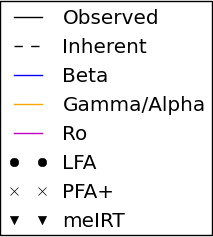
\includegraphics[width=30mm]{images/legend.png}
\caption{Legend for all figures in this section}
\label{fig:legend}
\end{figure}

\subsection{Missing KCs}
To see the impact on how many KCs were missing in each run of the experiment on each split it was noted during the experiment how many KCs were cleaned out from every part in a split and for how many KCs no variance was obtained because a KC was missing from too many parts. In table \ref{tab:kcmis} it can be seen how many KCs were missing on average (the splits were remade for every model). The number outside brackets is how many KCs were left out of that experiment completely. The number between brackets indicates how many KCs were on average missing from each part in the split of the experiment, including those that were left out of the experiment in the end. 

\begin{center}
\begin{table}[!htbp]
\begin{tabular}{| l | l|l|l|l|l|}

    \hline
    Splits & 6  & 8 & 12 & 16 & 32 \\ \hline
    Bridge &  87.3(90.1)& 85.7(99.7)& 88.0(121.2)& 87.7(137.1)& 89.3(190.4) \\ \hline
    Algebra & 7.3(8.5)& 6.7(8.9)& 6.7(11.5)& 7.0(14.0)& 7.7(21.3) \\ \hline
    Assistment & 0.7(1.2)& 0.7(1.1)& 1.0(1.3)& 1.0(1.8)& 1.0(5.7) \\ \hline

\end{tabular}
\caption{Average number of KCs left out of experiment with average number of KCs removed per split within brackets}
\label{tab:kcmis}
\end{table}
\end{center}

The KC's left out are quite constant in number; the increasing number of KCs missing per part as the parts get smaller is apparently off-set by the increasing number of parts. It does mean though that the second order variance of variances found would be higher than expected.

The number of KCs left out per dataset follows the same distribution of KCs left out per dataset in the initial cleaning which was seen in section \ref{sec:domain}. For the Bridge dataset the KCs removed form almost 20\% of the total KCs. Although it is unfortunate to miss this much data, it is a sign that for many KCs in this dataset too little data is available and that average variance of parameters would probably be worse when these KCs would be included. For the Algebra dataset the problem is small and for the Assistment dataset almost non-existent.

\subsection{Orderings within parameters}
To answer subquestion 2 from the research question rank orders were calculated between the different models build within each experiment. In figure \ref{fig:ranks} the resulting average tau values can be seen from all the experiments. The $\rho$ parameters of the PFA+ models show poor rank correlations over all datasets indicating that the rankings of this parameter are very invariant. This is a big disqualifier for the PFA+ model.
The tau values for the $\gamma$ parameter-type for both the PFA+ and LFA models are better, but still relatively low, the $\alpha$ parameter for the seIRT model does comparable on two datasets, but far worse on the third.
The $\beta$ parameter-type has the best tau values, good for the PFA+ and LFA models and worse, but still ok for the seIRT model.

\begin{figure}[!htbp]
\centering
\subfloat[Legend for the figures]{
  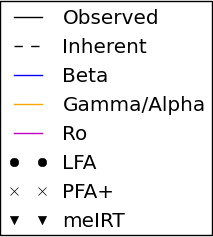
\includegraphics[width=30mm]{images/legend.png}
}
\subfloat[Rankorders for Bridge parameters]{
  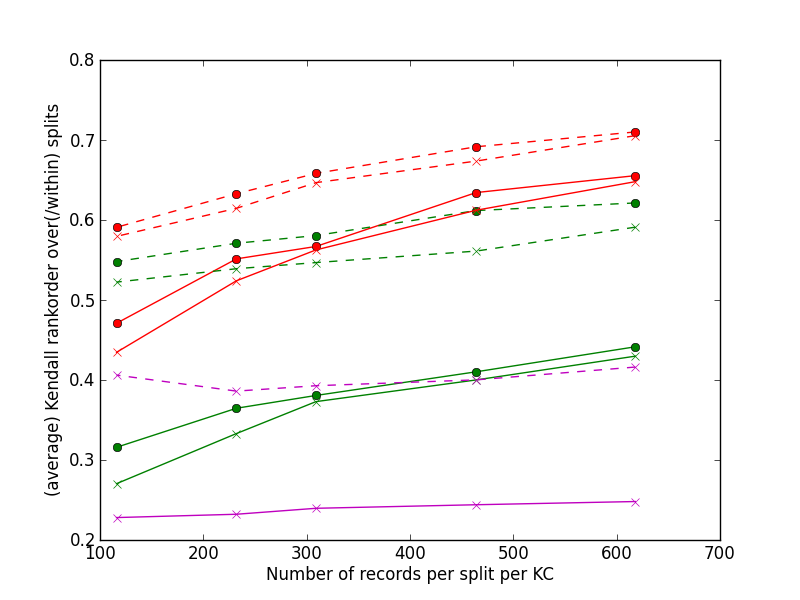
\includegraphics[width=65mm]{images/bridgeallmodranksKC.png}
}
\hspace{0mm}
\subfloat[Rankorders for Algebra parameters]{
  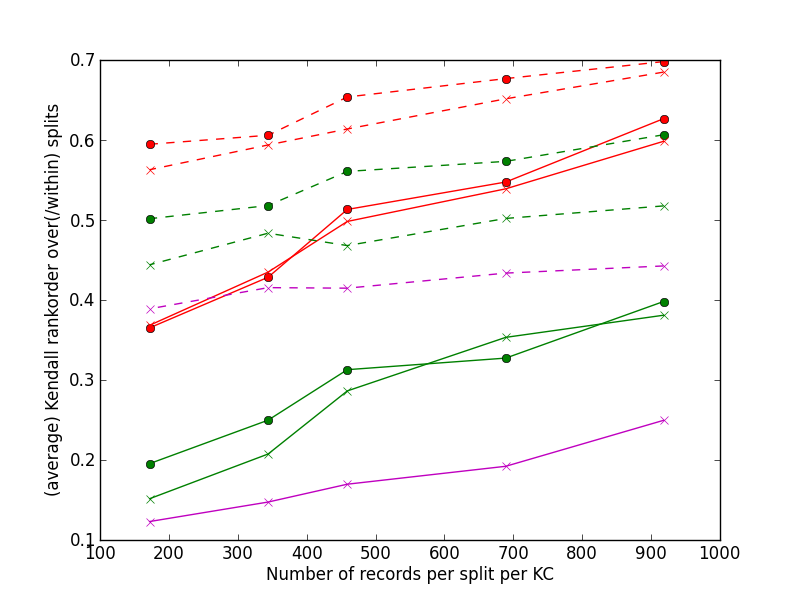
\includegraphics[width=65mm]{images/algebraallmodranksKC.png}
}
\subfloat[Rankorders for Assistment parameters]{
  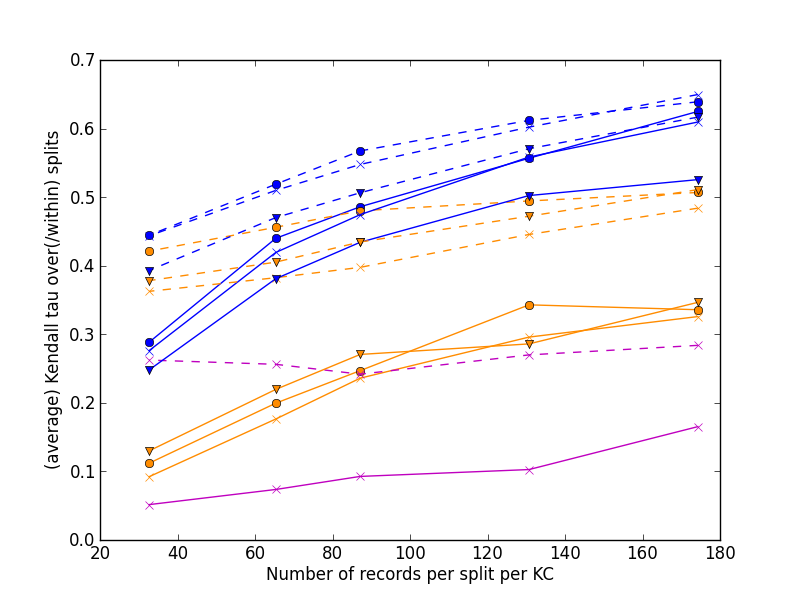
\includegraphics[width=65mm]{images/gongallmodranksKC.png}
}
\caption{Kendall's Tau rank orders of the different parameter-types}
\label{fig:ranks}
\end{figure}

The conclusion here is that the LFA and PFA+ models learning parameters ($\gamma$ and $\rho$) cannot be well distinguished and that these models can generally say little about relative learning speed of different KCs. The $\alpha$ parameters of the seIRT models are also poorly distinguishable. This parameter has an influence on the initial knowledge and learning parameters. It can thus be stated that the differences in initial knowledge and learning parameters in as far as they are based on the knowledge component are poorly distinguished. All models do distinguish between KC difficulties quite well, although the LFA and PFA+ models do this better than the eIRT model.

Figure \ref{fig:ranks} also holds information for the third subquestion concerning what the influence of data is on the invariance of the parameters. The hypothesis that invariance increases as more data is used holds across the board. There seems to be no direct relation between the number of records per KC used and the tau value, failing to give a rule of thumb of how much data is needed. Looking at the characteristics of the data, there is also no other measure of amount of data that would make an obvious candidate (e.g. number of students or student per KC) and it is surprising that the three figures look quite alike despite the different amounts of data used.

\subsection{Overall Invariance of Parameters}
\label{sec:varresults}
\subsubsection{Overall Variance}
To answer the mainquestion the average variance per parameter-type over all experiments is displayed in figure \ref{fig:sds}. To gain a better idea of the magnitudes of the standard deviations and to compare them across different parameter-types, each value is normalized by dividing them by the variance within the values of that parameter-type in a model fitted on the whole dataset.

\begin{figure}[!htbp]
\centering
\subfloat[Legend for the figures]{
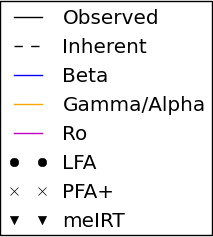
\includegraphics[width=30mm]{images/legend.png}
}
\subfloat[Standard deviations for Bridge parameters]{
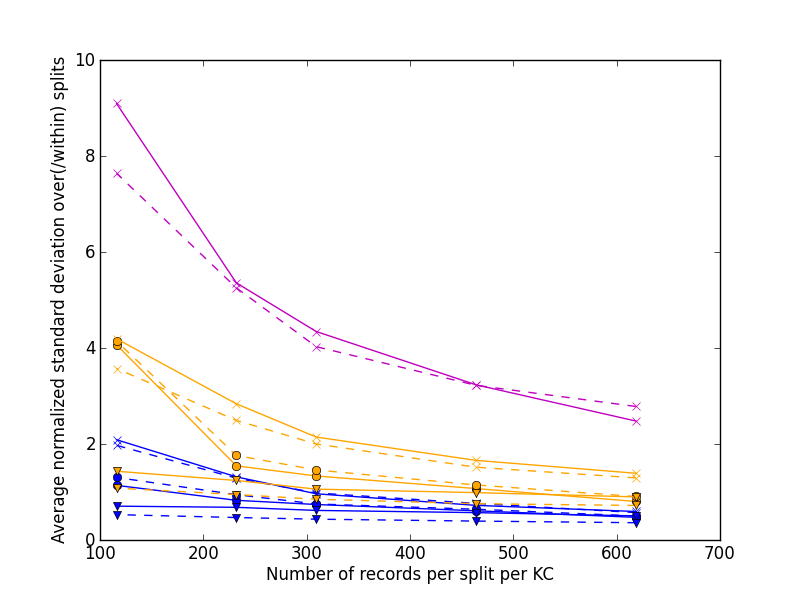
\includegraphics[width=65mm]{images/bridgeallmodsdsKC.png}
}
\hspace{0mm}
\subfloat[Standard deviations for Algebra parameters]{
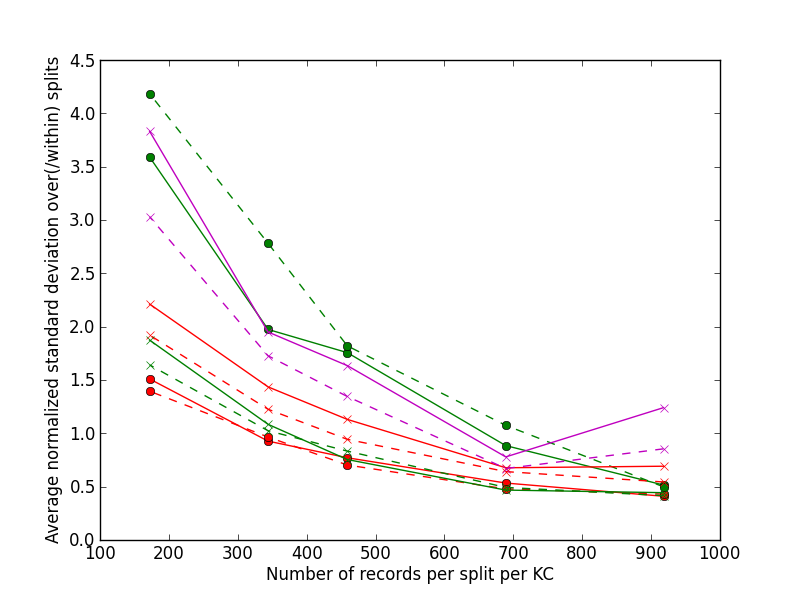
\includegraphics[width=65mm]{images/algebraallmodsdsKC.png}


}
\subfloat[Standard deviations for Assistment parameters]{
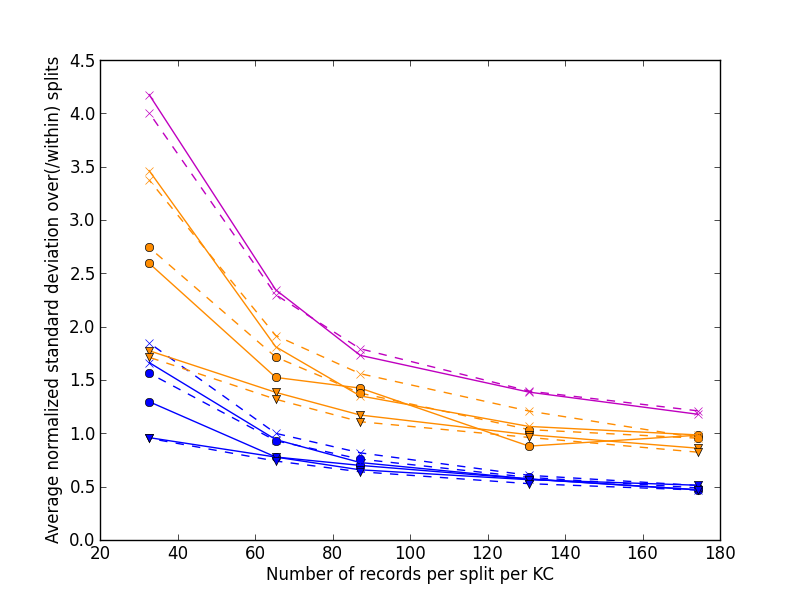
\includegraphics[width=65mm]{images/gongallmodsdsKC.png}
}
\caption{(Average) standard deviations of the different parameters}
\label{fig:sds}
\end{figure}

At first glance these results correspond to the results from the previous section. Some things jump out though: 1. the normalized variance, especially at splits where the parts have fewer data is extremely high 2. The difference between inherent variance and observed variance is generally low, while in the previous section the differences between the rankings were generally quite distinguished. 3. The ratio of variance of the parameters and the variance within a parameter-type should generally not be higher than 1. Investigating this problem let to the discovery that the general sizes of the parameters differ between experiments with splits into a different number of parts. The following subsection investigates this issue in more detail.




\subsubsection{Standard Deviation within Parameter-types}
\label{sec:parvar}
In order to see what happens to the parameter sizes of the parameter-types when using different amounts of data, figure \ref{fig:parvar} displays the average standard deviation of the parameter types in those experiments. Since this standard deviation also differs between models fit on real data and those fit on generated data these variances have been determined separately. Finally all values are divided by the standard deviation of that parameter-type in the model trained on all data (which was also used to normalize the values in figure \ref{fig:sds}). Due to the large values for some parameters, especially at parts with little data, a zoomed in version is displayed in figure \ref{fig:parvarz}. 
\begin{figure}[!htbp]
\centering
\subfloat[Legend for the figures]{
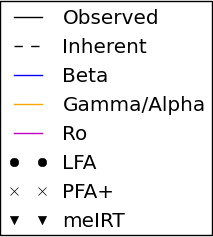
\includegraphics[width=30mm]{images/legend.png}
}
\subfloat[Standard deviations for Bridge parameters]{
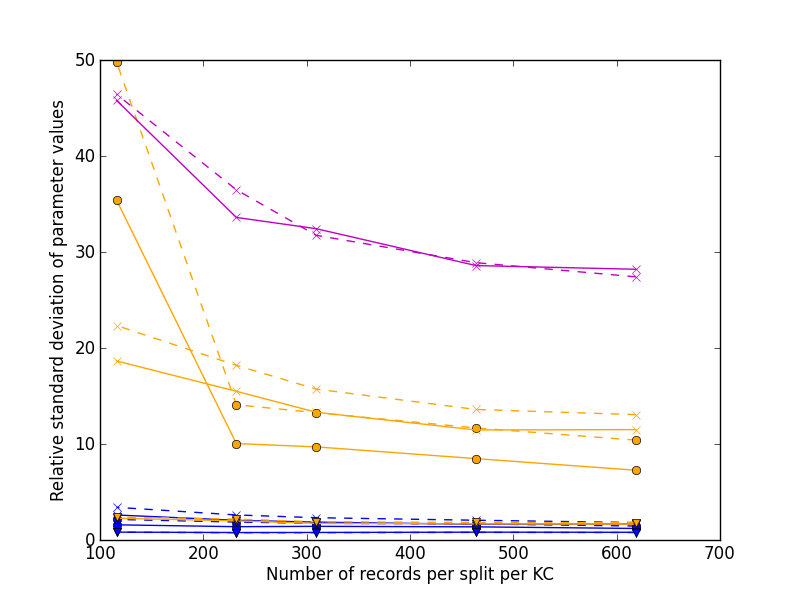
\includegraphics[width=65mm]{images/bridgeallmodsparvar.png}
}
\hspace{0mm}
\subfloat[Standard deviations for Algebra parameters]{
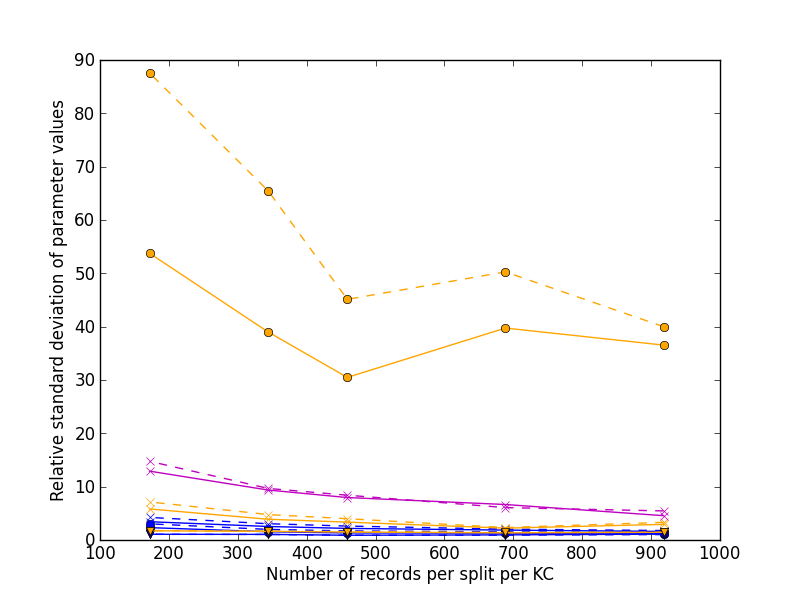
\includegraphics[width=65mm]{images/algebraallmodsparvar.png}
\label{fig:parvaralg}
}
\subfloat[Standard deviations for Assistment parameters]{
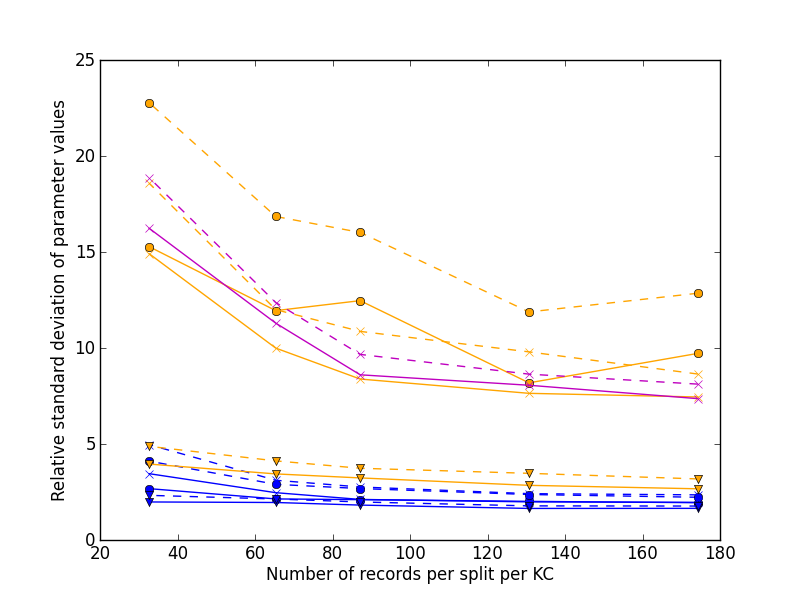
\includegraphics[width=65mm]{images/gongallmodsparvar.png}
}
\caption{(Average) standard deviations of the different parameters}
\label{fig:parvar}
\end{figure}



In figure \ref{fig:parvar} the high standard deviation within the learning parameter types of the PFA+ and LFA models are striking. A possible explanation for these results is overfitting: if for example a question for a KC is answered wrong a few times early on by some students, but mostly answered correctly after those initial questions, the model will fit a very high learning rate to this KC. If more students would be present whom might continue to sometimes answer questions concerning this KC wrongly, the KC would be fitted a substantially lower learning rate value. If this is the case it would mean that too little data was used here and that experiments with (seemingly much) more data should be done. Given that already quite a bit of data is used here, this does speak against how invariant the learning parameters of the PFA+ and LFA models are. It is expected that observed standard deviations reach 1 as data is increased up to the same amount as the original dataset. The steeper ascend might mean that increasing data beyond this point decreases the relative found variance below 1, indicating that even when using the whole dataset overfitting still occurs. It is thus not even certain that using the entire dataset is enough.

\begin{figure}[!htbp]
\centering
\subfloat[Legend for the figures]{
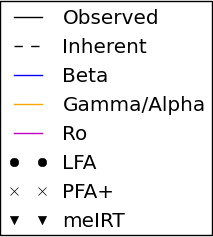
\includegraphics[width=30mm]{images/legend.png}
}
\subfloat[Standard deviations for Bridge parameters]{
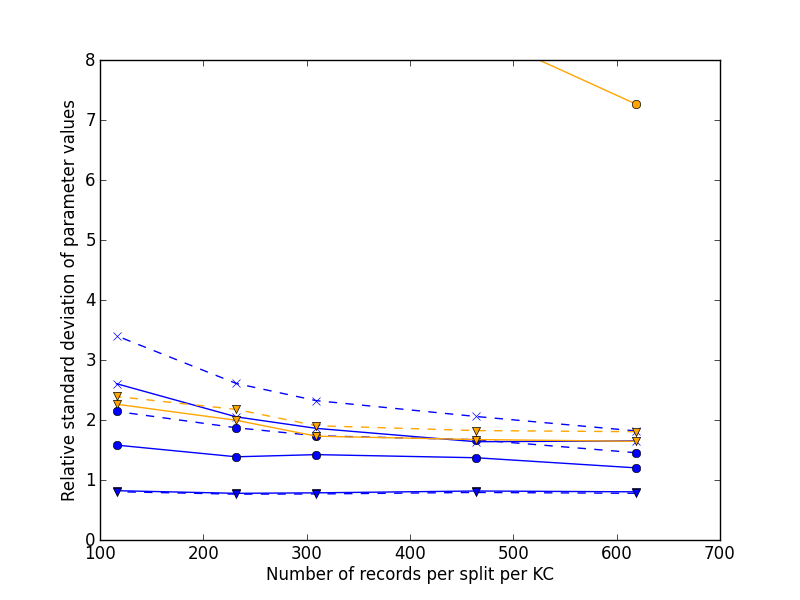
\includegraphics[width=65mm]{images/bridgeallmodsparvarz.png}
}
\hspace{0mm}
\subfloat[Standard deviations for Algebra parameters]{
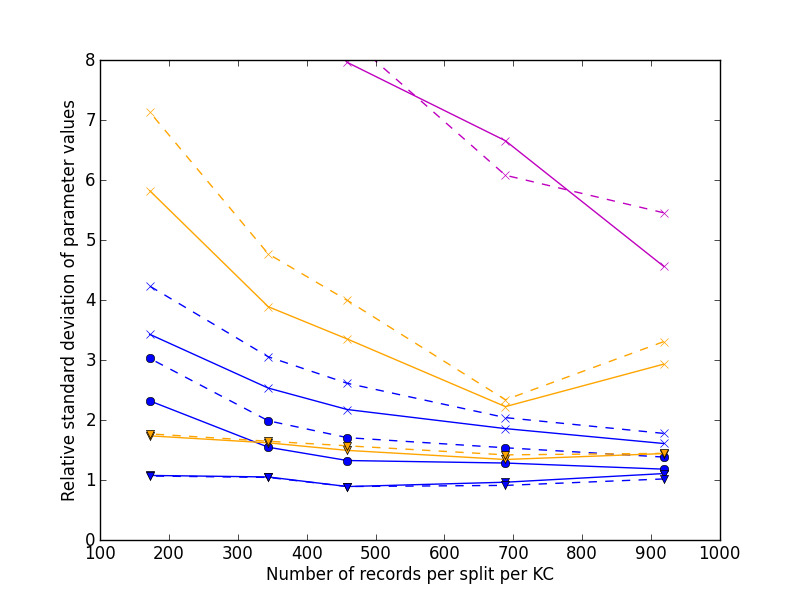
\includegraphics[width=65mm]{images/algebraallmodsparvarz.png}
}
\subfloat[Standard deviations for Assistment parameters]{
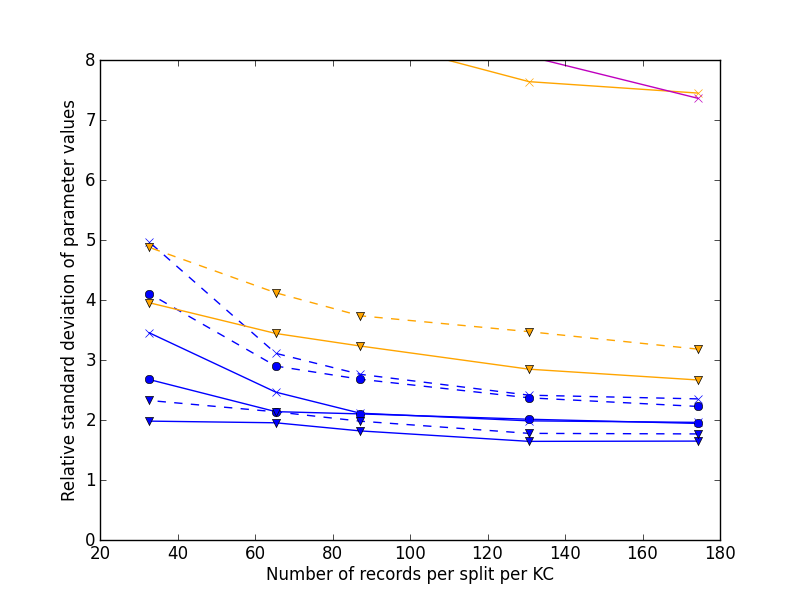
\includegraphics[width=65mm]{images/gongallmodsparvarz.png}
}
\caption{(Average) standard deviations of the different parameters}
\label{fig:parvarz}
\end{figure}

In figure \ref{fig:parvarz} it is visible that the parameters of the seIRT do much better in this regard, although less well for the Assistment dataset, indicating that more data is desired there. Also the $\beta$ parameters of the PFA+ and LFA models are fairly ok, indicating that overfitting is not so much a problem for them at higher amounts of data. Here too the issue is larger for the Assistment dataset, indicating the need for more data.

The standard deviations for the models fitted to simulated data are consistently higher than for those fitted on observed data. A possible explanation for this could be that overfitting continues to be a problem here, further increasing the size of parameters. Whichever is the case it weakens the basis of using simulated data to look at the theoretical variability of the parameters.

Finally there is a concerning issue visible in figure \ref{fig:parvaralg}: the $\gamma$ parameter-type of the LFA model has high standard deviations, but the $\gamma$ and $\rho$ parameters of the PFA+ model do not. It would be expected that if the $\gamma$ parameters of the LFA model the are actually overfitted, the $\gamma$ and $\rho$ parameters of the PFA+ model, with even less data per parameter, would be overfitted as well. No explanation for this discrepancy has been found.\todo{any ideas?!?}. 

\subsubsection{Adapted Normalization}
To account for the phenomena of increasing parameter sizes and still look at the standard deviation of parameters figure \ref{fig:sds} is repeated in figure \ref{fig:sdsalt}, but instead of using the variance in parameter-types of the model fitted on the whole data, the raw values from figure \ref{fig:parvar} are used to normalize the raw variances. This means that every datapoint has its own normalization factor instead of a single normalization factor for both the internal and observed variances of a model parameter at all different splits.

\begin{figure}[!htbp]
\centering
\subfloat[Legend for the figures]{
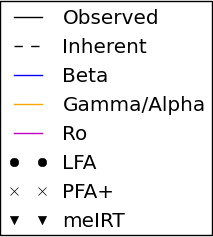
\includegraphics[width=30mm]{images/legend.png}
}
\subfloat[Standard deviations for Bridge parameters]{
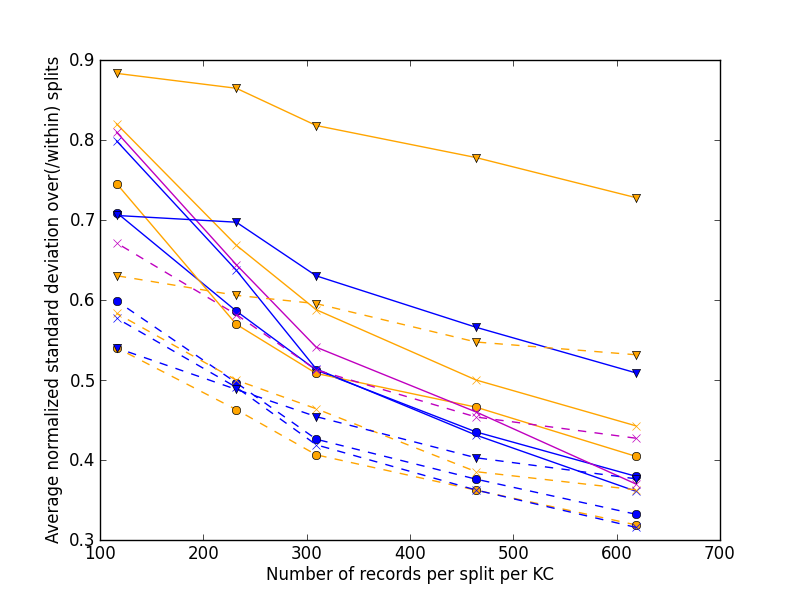
\includegraphics[width=65mm]{images/bridgeallmodsdsKCalt.png}
}
\hspace{0mm}
\subfloat[Standard deviations for Algebra parameters]{
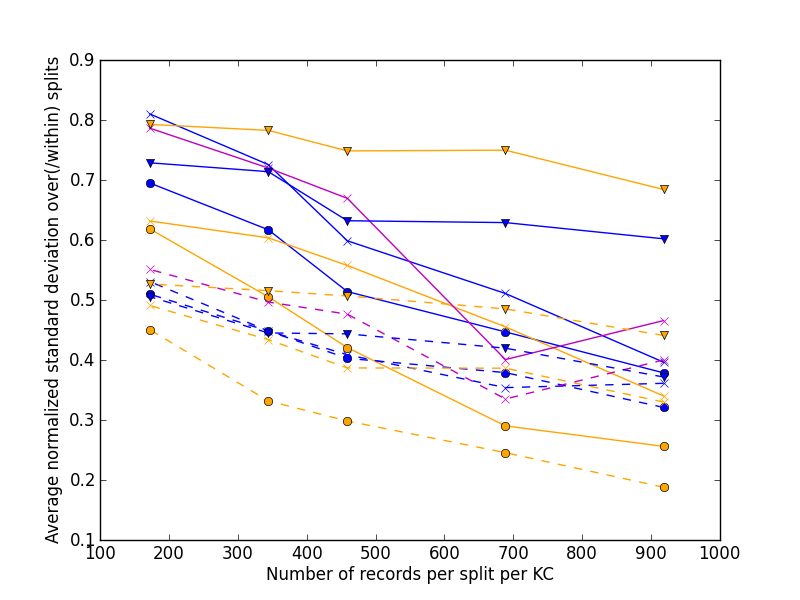
\includegraphics[width=65mm]{images/algebraallmodsdsKCalt.png}
}
\subfloat[Standard deviations for Assistment parameters]{
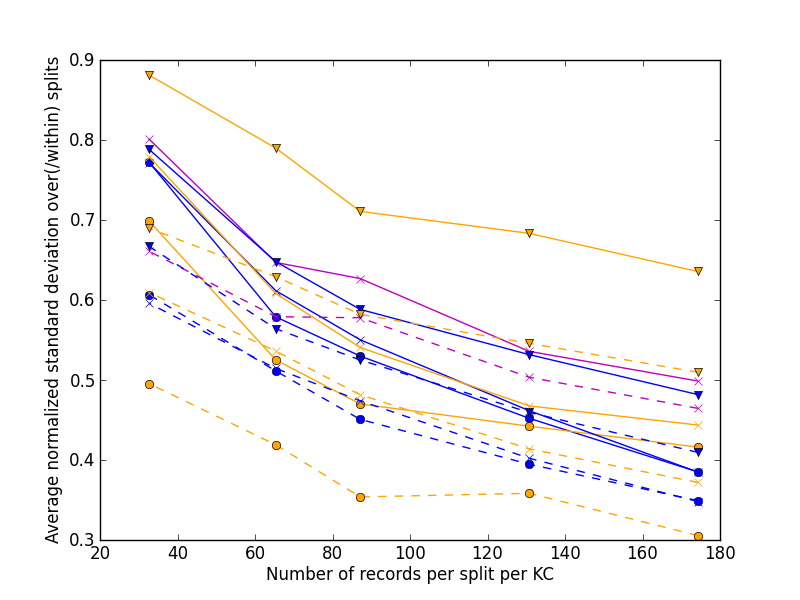
\includegraphics[width=65mm]{images/gongallmodsdsKCalt.png}
}
\caption{(Average) standard deviations of the different parameters}
\label{fig:sdsalt}
\end{figure}

In figure \ref{fig:sdsalt} the standard deviations of the parameters of the seIRT model are strikingly high. This is surprising since the tau values of this model aren't as bad. These contradictory results actually reinforce one of the reasons for using tau: the normalization step of the models parameters in the fitting procedure increase the found variance, while not meaning that the model is necessarily worse.

The discrepancy between figure \ref{fig:sdsalt} and the found tau values doesn't stop at the seIRT model. The $\beta$ parameters of the other models also seem to be doing relatively worse compared to the learning parameters of these models. The conclusions form this observation is that this method is biased towards parameter-types with high standard deviations. This conclusion is futher considering that in the Algebra dataset the $\gamma$ parameters of the LFA model scores well on this metric compared to the other parameters, while this parameter-type also had a high standard deviation. This section thus brings to light some major problems with parameter invariability of the AFM and PFA+ models, but fails to supply other useful information.

\subsection{Indicators of Variance}
To answer the fifth subquestion concerning an exploration of finding what measures might be used to predict the invariance of the parameters of a model. First the log likelihood and then A' are looked it, which are global measures of the model fit and thus only look at the global invariance. The last measure looked at is Inherent variance. Since inherent variance is given for every parameter, the relation between inherent variance and invariability of individual parameters can be investigated.

\subsubsection{likelihood}
In figure \ref{fig:likely} the points belonging to the different splits can easily be distinguished: there are three groups one for each data set (from left to right, Assistment, Algebra and Bridge) and within each group the point with the highest tau value is the one with the most data associated with it. That the PFA models have a higher likelihood is to be expected as it has more parameters than the LFA models. It is also sensible that with more data in a split the likelihood goes down, since the same number of parameter values is used to explain more data. Although there is a nice relationship between tau and likelihood within each dataset, this relationship probably stems from the previous two relationships mentioned: as the amount of data goes up, so do the tau values and as the amount of data goes up, the likelihood goes down. When looking over all three datasets there actually seems to be a slightly positive relation between likelihood and tau values. The wide spread of $\tau$ values over splits of the same dataset (where the relation is quite negative) compared to the slight positive relation makes it unlikely that likelihood can be used to make inferences about the distinguishability of parameter values.   

\begin{figure}[!htbp]
\centering
\subfloat[Average Log Likelihood vs Kendall Tau over splits]{
  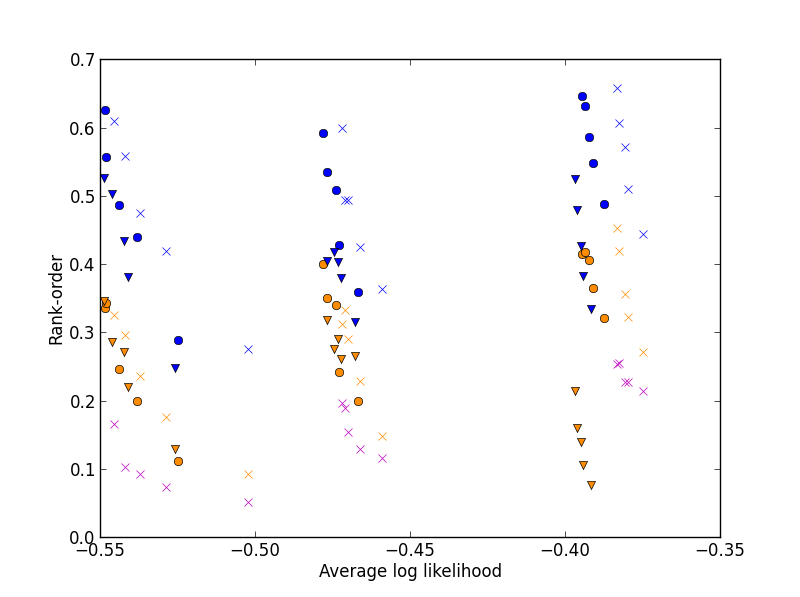
\includegraphics[width=65mm]{images/alllikely.png}
  \label{fig:likely}
}
\subfloat[a' vs total Kendall Tau over splits]{
  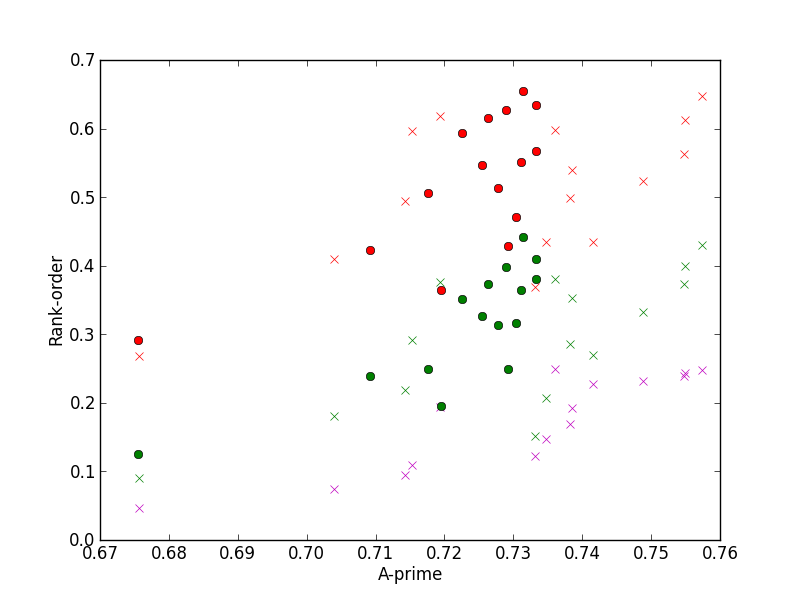
\includegraphics[width=65mm]{images/allaprimes.png}
  \label{fig:ap}
}
\caption{Kendall Tau values vs goodness of fit measures}
\end{figure}

\subsubsection{A'}
A' shows more promise to be a useful feature in establishing the invariability of orderings of parameter values. As seen in figure \ref{fig:ap} there is a positive relation between A' and the tau of each of the different parameters in both models. It should also be noted though, that A' might not be the best basis to favor one model over the other: PFA+ generally performs better on A+ than AFM, even though the the PFA+ model does worse when invariability of parameters is concerned.

\subsubsection{Inherent Variance}
The final measure looked at is the inherent variance. The inherent variance can be obtained on the whole dataset in contrast with the splitting method used. Initially the data from all splits of a model on a dataset were put together to obtain the spearman's rho values for each parameter-type. Discovering that variance within parameter-types is higher for splits with many parts for some models (as described in section \ref{sec:parvar}) caused some reconsideration of this approach. The issue is apparent when considering the usage of a rank-order correlation measure on a combination of two sets of paired values, one of which all values are between beteen 0 and 1 and the other where all values are between 1 and 2. The lack of overlap means that the rank-order correlation measure over the combined set is always better than the average of the measures of both sets. In this thesis an alternative method is considered to see how different the results would be. The alternative is to take the average rho value of the different sets.

In table \ref{tab:intorank} the Spearman's rho values are displayed. Outside the bracket is the rho value over the combined data from all the splits. The value within brackets is the average of the individual split experiments. Where the difference was .01 or less only one value is displayed. For 'Overall' the variance of all datasets were combined and one rho value calculated over them. The value between brackets is the average of the rho values of the different datasets.


\begin{center}
\begin{table}[!htbp]
\begin{tabular}{| l || l | l ||l|l |l||l|l|}

    \hline
     & LFA  & & PFA & & &seIRT &   \\ \hline
    Dataset & $\beta$ & $\eta$ & $\beta$ & $\gamma$ & $\rho$ & $\beta$ & $\alpha$  \\ \hline
    Bridge     & 0.86(0.82) & .92 & 0.91(0.87) & .95 & .92 & 0.68(0.65)&0.68(0.64) \\ \hline
    Algebra    & 0.90(0.87) & .97 & 0.92(0.90) & .98 & .96 & 0.70(0.64)&0.74(0.72) \\ \hline
    Assistment & 0.89(0.79) & .97 & 0.89(0.78) & .97 & .96 & 0.86(0.79)&0.88(0.83) \\ \hline \hline
    Overall    & 0.87(0.83) & .94 & 0.91(0.85) & .96 & .94 & 0.71(0.69)&0.72(0.73) \\
    \hline
\end{tabular}
\caption{Spearman's R of inherent vs total variance of various parameters and models over all splits (average instead of combination in brackets)}
\label{tab:intorank}
\end{table}
\end{center}



Mistery of rho values not in spaces where it would be expected.
\todo{Considering to throw this part out. It seems to add little, be a bit confusing and I realized for that I haven't used the adjusted standard deviations, which might be more sensible}


\section{Conclusion and Discussion}
\subsection{What is the standard deviation of the KC parameter values?}
The answer to this question remains largely undecided. In the cases of the PFA+ and LFA models the problem stems from the observation that parameter sizes increase as fewer data is used. In the case of seIRT the standard deviation seems to be estimated far too high, given that this model scores quite well on the invariability of parameter orderings. The observed increase in parameter sizes in PFA+ and LFA models makes this models poor candidates as this means that learning rates will be estimated as lower as more data is used.

\subsection{What is the invariability of the orderings within the KC parameter-types?}
The Kendall's Tau values show that the orderings of the learning parameters of the PFA+ and LFA models and the $\alpha$ parameter of the seIRT model vary considerably. Statements about some KC having a higher learning rate than another can generally not be made. In the case of seIRT it means that statements about differences between starting knowledge and learning rate of KCs can generally not be made. The exceptionally poor Kendall's Tau values for the $\rho$ parameters show that LFA should be preferred to PFA+ when invariability is desired.

\subsection{What is the influence of the amount of data on invariability?}
The hypothesis that with more data the variability of the parameters is reduced was confirmed. No straightforward relation between the amount of data and the standard deviation or Kendall's tau was observed over the three different datasets. For most parameters it seemed that improvement was still possible through adding more data. This improvement was relatively low and seemingly diminishing, leaving little hope for the Kendall's Tau values of learning parameters and the $\alpha$ parameter to improve to a useful level.

\subsection{To what extent is variability of parameters expected given the stochasticity of the model?}
On a globel level the inherent variance (represented as standard deviations) is quite close to the observed variance. On a micro level (of individual parameters) it is seen that the Spearman's Rho values between inherent and observed variance are high. Inherent variance as used here does seem a good indicator of variance of the paramter. There is one issue about the method used here: in cases where overfitting of parameter values seems to occur (resulting in relatively large value sizes), this problem is even worse for the calculated inherent variance.  

\subsection{Can the invariability of the model be indicated by other measures?}
The likelihood seems to hold no information on the invariability of the parameters. Since accuracy measures are often already looked at when considering learner models. Although generally better A' values do correspond with better invariability of rank orders, it is a bad idea to base model choice on this metric from an invariability of parameters perspective: PFA+ generally outperforms LFA, but has worse invariability of parameters.
\todo{considering to here only look at A' as a measure used to evaluate models and do this different in the results to match the new question. The part on spearman's rho will than only belong to the prevous section}  

\subsection{Improvements}
The results for the standard deviations were quite poor and inconclusive. Using the standard deviation within parameter types can probably be improved by using the absolute sum of all parameters of a type for normalization. This is because parameter size and standard deviation are definitely related (double the parameter sizes and the standard deviation doubles as well), but a doubling of the standard deviation, doesn't mean that the parameter sizes on average have doubled. Using this method could potentially get rid of the problem that parameter-types with high standard deviations benefited disproportionately from the adapted normalization.

The standard deviations and Kendall's tau values in which the results are represented are hard to interpret. A solution could have been to take some ITS scenarios (some questions to some students for every KC) and then see how much the different values of the parameters in the different parts would have mattered at the end. Besides giving more interpretable results this would also remove the indeterminacy issue of the seIRT model that is thought to increase the observed variance of its parameters.



\subsection{Further Research}
Amount of data in this research was looked at from a global and crude perspective. Instead it would be good to look at a low level at how much data is necessary concerning a particular KC to make the parameter estimates for that KC accurate. The effect of multiple KCs being associated with an item should also be considered.

The method to obtain inherent variance should be looked into further. The 'overfitting' (if that is what happens) should be investigated and perhaps the difference between inherent variance and observed variance can be used to indicate when this overfitting no longer occurs.

The method used to investigate the invariability of the parameters did not use Hambleton's idea of selectively splitting the data. This path should be explored further. For example splitting the students by skill may show that in the LFA and PFA+ models learning rates are high for the high skill group and low for the other and show holding the learning rate independent of students is too strong an assumption. Making the split based on difficult versus easy KC's (which is less trivial!) and using model where the learning rate is solely dependent on the student it could be seen how important the assumption that the learning rate is dependent on the KCs is. 

\todo{Some final words? Final other stuff}

\bibliographystyle{alpha}   % this means that the order of references
			    % is determined by the order in which the
			    % \cite and \nocite commands appear
\bibliography{litlist}
\newpage
\appendix
\section{Implementation and Mathematical argumentation}
\label{app:math}
The LFA and PFA models are relatively straightforward in their data representation and implementation. For these models $x$ in formula \ref{eq:logistic} is linear in the parameters, which means that standard logistic regression can be applied. In this appendix first the way the data is represented is described followed by a proof that logistic regression indeed finds the parameter values where the likelihood of the data is highest. 
\subsection{Data Representation}
For logistic regression the data is represented in a matrix $\Phi$ such that $\Phi w$ is equal to a vector of each value of $x$ in formula \ref{eq:logistic}, where $w$ is a column vector of the parameter values. 
In this matrix the rows represent data points while the columns represent what the parameters should be multiplied with. The dimensions of the matrix are thus equal to the number of data points by the number of parameters.

In the formulas for the LFA model (formula \ref{eq:afm}) and the PFA model (formula \ref{eq:pfa}) $x$ consists of a sum where every part contains exactly one parameter. This makes construction of $\Phi$ straightforward: in each row (thus for every data point) a 1 is placed for every present parameter that stands isolated (this goes for $\theta$ and $\beta$) and for the others ($\eta$,$\gamma$ and $\rho$) the right value for that data point is inserted (a non-negative integer). Any parameter not used for that specific datapoint will have a value of 0.

\subsection{Workings of Logistic Regression}
Logistic regression estimates the values of the parameters that maximize the likelihood of the data given the model. The likelihood of the data is equal to $\prod_{d \in D} P_{d}^{t_d}  (1- P_{d})^{1-t_d} $. Here $D$ is the set of all data points and $t_{d}$ is the label (0 for incorrect, 1 for correct) of data-point $d$. The logarithm of this function is taken as this will retain a maximum at the same parameter values, while being easier to derivate since we now have a sum instead of a product. Finally the negative of this log likelihood is taken as this is slightly easier to work with, which results in a minimum being looked for rather than a maximum. The function is then $-\sum_{d \in D}(t_{d} ln(P_{d})+(1-t_{d}) ln(1-P_{d})$.

The first step in finding a solution to this minimization problem is taking the first derivatives of this function in all the parameters. The logistic function has the practical characteristic that its derivative in $x$ is $\sigma (x) (1- \sigma(x))$. The whole derivision can be seen in formula \ref{eq:der1}. Here $\phi_{d}$ is the data for data-point $d$ and is introduced as the derivatives of $x$ in all the parameters. This is possible as $x$ is a linear function in all the parameters. The second to last step is only possible since t can only be 1 or 0. 

\begin{equation}
\label{eq:der1}
\begin{split}
-\sum_{d \in D}(t_{d} \frac{1}{P_{d}} P_{d} (1-P_{d})\phi + (1-t_{d}) \frac{1}{1-P_{d}}(1-P_{d}) (1-(1-P_{d}))(-1)\phi_{d}) &=  \\
-\sum_{d \in D}(t_{d} (1-P_{d})\phi + (1-t_{d})(1-(1-P_{d}))(-1)\phi_{d}) &= \\
-\sum_{d \in D}(t_{d} (1-P_{d})\phi + (1-t_{d})(-P_{d}))\phi_{d}) & = \\
-\sum_{d \in D}(t_{d}-P_{d})\phi_{d} &= \\
\sum_{d \in D}(P_{d}-t_{d})\phi_{d} &
\end{split}
\end{equation}

The first derivatives would be sufficient to perform gradient descent, but this introduces the complexity of finding the right step-size (function). The Newton-Raphson method is an alternative, which can find the parameters where all the first derivatives are 0. For Newton Raphson it is necessary to find the derivatives of the functions we are want to reach zero (i.e. we need all the second derivatives, which is the Hessian). The Hessian is straightforward to obtain as $\sum_{d \in D}(P_{d} (1-P_{d}) \phi^{T}*\phi)$ where $\phi$ is seen as a row vector. Now the second derivative can be written as a single matrix multiplication: $\Phi^{T} R \Phi$ where $R$ is a diagonal matrix with $P_{d} (1-P_{d})$ on the diagonal. Now the Newton-Raphson method can be applied to find a minimum to the -log likelihood of the data.

Simply finding a minimum is not enough. We want to be sure that we actually find the minimum. In the case of logistic regression there is only one minimum and this must thus be the minimum that is found. The reasoning as to why this is true is explained in this paragraph. That the minus log likelihood has only one minimum is because it is a convex function and a convex (twice differentiable) function always has a semi-definite Hessian (and vice versa). For the Hessian to be semi-definite it is required that for any possible real valued vector $x$, $x^{T}Hx\geq 0$. In the previous paragraph it was established that the Hessian in this case is $\Phi^{T} R \Phi$. Taking $a=\Phi x$ we are left with $a^{T}Ra\geq 0$ as the necessary condition for the Hessian being semi-definite. Since the left side of the equation turns into a sum of squares multiplied by elements from R (which are all zero or positive), this equation must hold. The minus log likelihood is thus a convex function and a found minimum must be the global minimum.

\begin{comment}
\pagebreak 

\section{Glossary}
\todo{
Making a start with using terms consistently, plus I generally feel that a glossary would have helped me greatly in understanding papers etc.}
\begin{description}
\item[Answer]Whether a question was answered correctly or incorrectly
  \item[Item] A problem (step) in the ITS to which a single answer can be given
  \item[Knowledge Component] A skill, piece of knowledge etc. that is associated with one or more items and in which students can have a level of competence (named 'skill' here)
  \item[paramater] A type of parameter used in one of the models (e.g. $\beta$)
  \item[paramater value] The value of a parameter belonging to a specific case (e.g. the value of the $\theta_{0}$ parameter belonging to student number 10)
  \item[Question] An instance of an item, as asked to a single student
  \item[Skill] Level of skill of a single student
\end{description}
\end{comment}
\end{document}
